%%% Local Variables:
%%% mode: latex
%%% TeX-master: t
%%% End:

\documentclass[master,openright]{tongjithesis}
% \documentclass[%
%   master|doctor, % mandatory option
%   xetex|pdftex|dvips|dvipdfm, % optional
%   secret,
%   openany|openright,
%   arialtoc,arialtitle]{tongjithesis}

% 所有其它可能用到的包都统一放到这里了,可以根据自己的实际添加或者删除。
\usepackage{tongjiutils}
\usepackage[top=2.54cm, bottom=2.54cm, left=3.17cm, right=3.17cm]{geometry}

% 你可以在这里修改配置文件中的定义,导言区可以使用中文。
\def\myname{邱君诚}

\begin{document}

% 定义所有的eps文件在 figures 子目录下
\graphicspath{{D:/mthall/}{figures/}}

%%% 封面部分
\frontmatter

%%% Local Variables:
%%% mode: latex
%%% TeX-master: t
%%% End:
\secretlevel{保密} 
\secretyear{2}

\ctitle{电容式离子电流检测电路的离子电流适用工况拓展}

% 按照申请工学学位设计。如有其它需要,请修改相应文字。
\makeatletter
  \iftongji@doctor
    \cdegree{工学博士}
  \else
    \iftongji@master
      \cdegree{工学硕士}
    \fi
  \fi

\makeatother

\cdepartment{汽车学院}

\cmajorfirst{动力工程}

\cmajorsecond{}

\cauthor{邱君诚}

\cstnr{1335034}

\degtype{工学}

\csupervisor{吴志军 教授}

% 如果没有副指导老师或者联合指导老师,把各自{}中内容留空即可。

\cassosupervisor{}

\ccosupervisor{}

% 日期自动生成,如果你要自己写就改这个cdate
%\cdate{\CJKdigits{\the\year}年\CJKnumber{\the\month}月}
\makeatletter
  \iftongji@doctor
    \edegree{Doctor of Philosophy}
  \else
    \iftongji@master
      \edegree{Master of Science}
    \fi
  \fi

\makeatother

\cfunds{}

\efunds{}

\etitle{Condition Expand on Ion Current Characteristics Based On Capacitive Detection Circuit}

\edepartment{School of Automotive Study}

\emajorfirst{Power Machinery and Engineering}

\emajorsecond{TONGJILUG}

\edispline{Engineering Science}

\eauthor{Juncheng Qiu}

\esupervisor{Prof. Zhijun Wu}

%\eassosupervisor{Prof. Gang Wan}

% 这个日期也会自动生成,你要改么?
% \edate{May, 2009}

% 定义中英文摘要和关键字
\begin{cabstract}
电容式离子电流检测电路具有性价比高,安装方便的特点。但是由于没有屏蔽点火干扰,随着转速的增加,容易造成点火干扰淹没正常的离子电流信号的弊端。\par
本文通过小波分析的方法很好的将离子电流信号中的点火干扰信号分离出去,获得了理想的离子电流信号。同时比较不同的小波基函数以及小波分析层级,得出了最佳的小波基函数和分解层数。离子电流的火焰后期
信号在理论上近似高斯函数,同时缸内的循环废弃导致的离子电流信号也可以近似成高斯函数,整个检测到的离子电流信号可以用双高斯曲线进行拟合。
采用了拟合算法得到的拟合曲线参数,能够快速地计算出离子电流的各种特征值,能够大大缩小需要的发动机控制系统的计算资源;比较了特征值的估计值和真实值之间的相关性和循环波动率,验证了
双高斯曲线拟合算法估算离子电流特征值的有效性。\par
离子电流的火焰后期开始时刻估计值与结束时刻估计值、最大离子电流升高率估计值与各自对应的特征值有一定的相关性。
离子电流的火焰后期峰值相位估计值、离子电流积分值估计值和最大离子电流升高率相位估计值与各自对应的特征值有明显的相关性。
离子电流积分值和升高率估计值有一定波动,其他特征值的估计值都具有很好的稳定性。
\end{cabstract}

\ckeywords{离子电流, 点火干扰, 小波分析, 高斯曲线}

\begin{eabstract}
Capacitive detection circuit has cost effeciency and is easy to deposit. 
But due to the ignition interfere, the ion current would be submerged by the interfere with the engine speed up.
This is a weak point of this kind of ion current detection circuit.\par
In this paper, real and ideal ion current is extracted
using wavelet analysis method. Different wavelet functions are compared and different wavelet are discussed to dertermine
the best wavelet function and wavelet level. The profile of real ion current in post-frame peroid is similar to that of 
gaussian curve, and the ion current caused by residual waste gas of last cycle also has the similar profile to gaussian
 curve. So the whole ion curren could be simulated by the addition of two gaussian curves and eigen value of ion current
 can be calculated fast by the parameters of two gaussian curves conviniently reducing the computing resource of engine control 
 system. The coefficience of estimated value of each eigen value to each eigen value is validated and fluctuation ratio 
 of each eigen value is calculated to determine the application of double-gaussian method.\par
The time of start and end of post-frame period, the maximum ion rising rate has certain
correspondence to each corresponding eigen value. Ion peak phase, ion integeration and maximum ion
rising rate phase has explicit correspondence to each corresponding eign value.
Despite ion integration and ion rising rate, all the other estimated value have good solidity.
\end{eabstract}

\ekeywords{Ion Current, Ignition Interfere, Wavelet Analysis, Gaussian}

\makecover


% 目录

\tableofcontents

% 符号对照表
\begin{denotation}
\item[GNU] GNU's Not Unix /'gnu:/
\item[GFDL] GNU Free Documentation License
\item[GPL] GNU General Public License
\item[FSF] Free Software Foundation
\item[SMP] �Գƶദ��
\item[API] Ӧ�ó����̽ӿ�
\item[$E$] ����
\item[$m$] ����
\item[$c$] ����
\item[$P$] ����
\item[$T$] ʱ��
\item[$v$] �ٶ�
\end{denotation}


%%% 以下索引按需要选择
% 插图索引
%\listoffigures
% 表格索引f
%\listoftables
% 公式索引
%\listofequations
\cleardoublepage
%%% 正文
\mainmatter
\chapter{绪论}
\section{前言}
早在十九世纪,人们就观察到碳氢化合物在燃烧时会产生自由离子,使得火焰和燃烧产物具有导电能力。这一现象被注意到,
并逐渐运用到燃烧过程研究工作。在火花塞点火式发动机中,当燃烧发生时,火花塞电极之间就产生大量的离子。如果在火花塞
两极之间加上适当的直流偏置电压就会形成离子电流,通过该电流可以对发动机进行检测实现对发动机的实时监测。但是,由于
以往对发动机控制技术要求不高,同时受发动机控制软、硬件系统的整体技术水平限制,该方法并未引起人们的广泛
注意。近年来,随着对发动机效率及排放性能要求的逐渐提高,该方法逐渐引起重视。离子电流检测技术的最
初应用主要是面向于失火现象的检测,在美国国家环保局(EPA)第II代车载诊断装置(OBDII)法规颁
布后,要求在所有负荷和转速下实现100\%失火检测\cite{grzys}。世界上许多厂家采用的是曲轴转速波动法,但这种方法在
路况较差的情况下会产生干扰信号,影响检测结果,而采用离子电流法则可以避免上述问题,实现100%失火检测。由此,对离子
电流检测技术的研究逐渐由对燃烧过程中的失火、爆震等现象的定性检测,逐渐向空燃比、燃烧相位及缸内燃烧压力状态等参数的定量检测上来。
\section{国内外研究现状}
目前,对离子电流检测技术的研究主要集中于离子电流的形成机理、应用途径、特征提取及参数估计方法以及实际控制应用等四个方面。
\subsection{离子电流的形成机理研究}
早在1953年Winch和Mayes\cite{winch1953method}就利用了偏置电压式的离子电流检测电路记录了离子电流信号,并以此分析了缸内燃烧状况。在20世纪
50年代,出现了大量的研究火焰中化学离子平衡和火焰后燃区的研究成果。进入80年代,汽车领域的科技工作者致力于离子电流信号的研究,取
得了很多重要的成果。1986至1997年Nick Collings\cite{collings1986knock,collings1991plug,collings1985knock}发表了利用火花塞作为传感器检测爆震的三篇论文,介绍了离子电流
法的基本原理和离子电流的发展历程,并完善了爆震检测的方法。1996年Andre Saitzkoff\cite{saitzkoff1996ionization}发表了火花塞离子电流的平衡计算的论
文,利用偏置电源式离子电流检测电路测量了离子电流信号,通过分析得到了火花塞离子电流的近似理论计算公式。2000年Wayne University
的D. Schneider\cite{schneider2000experimental}发表了离子电流与内燃机工作参数之间关系的博士论文。

在离子电流的形成机理研究方面, Saitzkoff和Reinmann等人\cite{saitzkoff1996ionization}率先对$N_{2}$,$H_{2}O$,$CHO$和$NO$四种基团在离子电流形成过程中所起的作用
进行了对比分析。研究认为燃烧火焰电离后能够定向移动的自由离子只占极小部分,其原因在于移动能力上的差异。同时,研究表明占离子总浓
度1%的$NO$基团产生离子电流的能力最强。Kessler等人\cite{kessler}在柴油机上采用光学方法对离子电流的研究表明,由于柴油和汽油在燃烧时产
生自由离子的化学反应过程不同,二者产生的离子电流信号波形差异显著。在汽油机上形成的离子电流中,电子是负电荷的主要载体,而对于
柴油机上的所形成的离子电流,带负电的离子也需考虑。A.Franke\cite{franke2003analysis}在对汽油机离子电流产生的物质来源的分析基础上,首次将离子
电流的产生划分为火焰前锋期和火焰后期两个阶段,认为在火焰前峰期的离子电流主要是由火焰前锋面与火花塞电极接触时所产生的,而
在火焰后期热电离过程是形成离子电流的主要原因。

除了离子电流产生的化学动力学机理外,气缸结构及火花塞位置等物理因素也是影响离子电流波形的重要成因。L.Peron等人\cite{peron2000limitations}对离子电流
信号的局限性分析认为,离子电流生成机理并不是决定信号波形的唯一原因。
\subsection{基于离子电流的检测应用研究}
目前对离子电流的应用已经从初期对失火及爆震的定性研究转入对燃烧参数的定量研究。在空燃比检测方面,Reinmann\cite{reinmann1997local}利用离子电
流公式理论和实验论证拟合了空燃比-离子电流公式。Kenneth Ratton和Ming C. Lai等人\cite{balles1998cylinder}利用火花间隙电离检测研究了缸
内空燃比的近似值,观察到了空燃比和离子电流特征之间的较强相互关系。其研究认为,从整体性能上看,离子电流检测无法取代缸压检测,二者
信号质量和性质都完全不同。但通过具体工况下对离子电流波形的具体分析,该方法仍具备有对空燃比进行实时反馈的潜力。在对缸内燃烧
压力状态的检测方面,Chao.F等人\cite{zhu2003mbt}提出,部分负荷工况下,对离子电流信号进行了多循环平均处理,通过处理后信号的第二峰位置
及幅值,实现了对缸内燃烧峰值压力及其位置的准确预测。
\subsection{特征提取及参数估计算法}
在基于离子电流的燃烧特征提取算法方面,J.Forster等人\cite{forster1999ion}率先基于离子电流的频域特征,实现了对爆震及其强度的准确估计。该研
究展示了爆震强度与离子电流频域信号高频区域内幅值的相关性。此后,一系列针对产品发动机爆震检测的相关研究也相继出现。这些研究
中普遍采用了离子电流的频域特征实现了较高质量的爆震检测。

此外,Gerard等人\cite{malaczynski2003real}针对不同燃烧边界条件下,离子电流信号变化规律复杂的情况,提出了基于信号时域特征,采用主成分分析方
法对离子电流信号进行了特征提取,该方法可以有效的对离子电流信号观测窗内观测样本进行降维,从而减小后续的参数估计算法的计
算量。

在基于离子电流的参数估计方法方面,由于离子电流信号的产生机理复杂,信号波形变化规律多样,在利用该信号进行燃烧特征检测时
,大多采用了数学模型来建立电流信号特征与被估参数之间的映射关系。在这方面,Gazis等人\cite{panousakis2006ion}通过双高斯曲线拟合的方法,对电流
信号的时域特征进行了提取,并针对离子电流信号的非线性变化特征,采用神经网络方法实现了对汽油机燃烧峰值压力位置的准确预测。
\subsection{基于离子电流反馈的实时控制}
Magnus等人\cite{glavmo1999closed}在研究柴油机EGR和颗粒污染对离子电流的影响时,尝试了在稳态工况下,通过多循环均值后的离子电流信特征值
号对燃烧始点进行反馈和控制。先预定一个离子电流信号强度阈值,当检测到的离子电流信号首次越过该阈值时,该时刻被定义为燃烧
始点。对燃烧始点检测成功后,可以通过调整燃油十六烷值和空气、燃油以及发动机温度等相应方法,对滞燃期加以调整。
\subsection{国内研究现状}
在国内许多科研院校和研究所针对离子电流也展开了大量的研究工作,其中典型的诸如,同济大学李理光课题组\cite{dgy2011,zqy2011,fqw2012,zzybh2012,cyb2013}针对汽油机的点燃方式和
均质压燃方式下离子电流的产生机理及信号特征变化规律进行了研究,分析了两种燃烧模式下信号的产生机理及影响因素。在此基础上,研
究了基于该信号的特征提取及燃烧信息反馈方法。进而,针对现有发动机传感及控制方法的不足,提出了以离子电流信号为反馈量,在发
动机上实现基于循环的燃烧信息反馈及控制思想。西安交通大学的吴筱敏\cite{gh2010}和天津大学的谢辉等课题组也基于离子电流检测手段进行汽
油机爆震、空燃比检测和燃烧相位判断等相关研究。
\section{本课题的意义和主要研究内容}
常见的离子电流检测电路分为电容式和偏置电源式。偏置电源式检测电路可以将点火干扰屏蔽,获得的离子电流曲线便于分析计算\cite{cyb2012},但
是由于需要使用高压硅堆和外置电源成本太高。电容式检测电路结构简单,成本低廉,但是点火干扰阶段容易和火焰前锋期甚至包括焰后期重
叠,导致离子电流的一些特征参数无法识别。如果能够提出一种较好的信号处理方法处理点火干扰阶段信号,将会使成本低廉、结构简单的电容
式检测电路得到推广。
\par 正常情况下,采用电容式离子电流检测电路得到的离子电流信号曲线可以分为三个时期;火花塞放电期,火焰前锋期,火焰后期。火花塞放
电期间,由于次级线圈放电导致检测电路中产生了较大的电流。但如果火花塞附近发生早燃,则在点火信号之前或之后将产生一些峰值\cite{eriksson1997closed}。如
果火花塞点火放电时间过长,将会和火焰前锋期甚至是火焰后期的离子电流信号重叠,从而影响了离子电流信号的分析。
\par 在重叠情况下,仍然可以预估甚至提取离子电流。由于点火干扰的根本原因是点火能量在点火线圈中的震荡,其频率是有一定规律的。火焰前锋
期的电流信号主要和火焰传播过程相关,火焰后期的电流信号和缸内的热力学过程相关,这两个时期的电流信号频率和点火线圈中的能量震
荡频率区分明显。这是离子电流被淹没而仍然可以预估甚至提取的基本原理。所以为了能够准确地提取离子电流信号,首先需要通过对电容式
离子电流检测电路和纯点火干扰信号进行分析,以便了解点火干扰信号的频幅特性。而在失火情况下,由于燃烧没有发生,离子电流信号没有产生。所以
失火是检测电路测定的信号就是纯点火干扰信号。除了信号提取的方法之外,Saitzkoff\cite{saitzkoff1996ionization}做了很多研究,提出了近似的离子电流计算公式。通过将
这些公式进行简化提出一些参数函数,也能够很好的预测离子电流的波形和特征参数,甚至可以达到预测空燃比的要求。
\par 离子电流的火焰前锋期信号是由于燃烧的火焰前锋造成的,所以该时期的离子电流能够很好的用于分析缸内的燃烧状况,比如计算燃烧锋面的速度。而
离子电流的火焰后期是由于火焰前锋面已经离开火花塞电极,但是缸内燃烧仍在继续,导致的缸内热力学变化引起的热电离而形成的,所以能够很好的反映内燃机的负荷,缸内压力变化等。
\par 所以正确地获得离子电流两个时期的信号曲线对于分析缸内的燃烧情况是非常重要的。但是这两个时期的信号极容易被点火干扰信号淹没,导致无法得到
准确的离子电流信号。通过上述的一些方法去除干扰信号,就可以帮助更好的认识离子电流信号,为后续的研究扫清障碍。即使无法完整准确地消除点火放
电干扰信号,仍然能够通过上述方法统一处理每个循环的离子电流信号,得到该处理方法下的某个稳定的特征变量,从而指导反馈控制发动机的运行参数。

\chapter{数值模型的理论基础}
数值模拟已经成为内燃机设计开发和优化过程中的一个重要研究手段。由于内燃机工作过程中缸内形成高温和高压的环境
现有的测试方法很难直接将传感器安装在缸内进行测量,因此数值模拟在内燃机工作过程的研究上得到了广泛应用。
\section{离子电流模型}
点燃式内燃机在燃烧过程中,产生大量的化学反应,在缸内会产生大量的带电粒子\cite{ljwwty2008},并且这些带电粒子的运动具有无规律的特性。
如果在火花塞两级施加一个稳定的直偏电压,由于有外加电场存在,带电粒子发生定向迁移,从而形成了火花塞离子电流。\par
以下的离子电流模型是基于以下的几个假设而成立的:
\begin{itemize}
\item 火花塞间隙中的燃气完全燃烧
\item 燃烧过程满足绝热过程
\item 燃气满足热力学平衡
\item 火花塞间隙近似成圆柱模型
\end{itemize}
\subsection{缸内燃烧化学反应式}
通常认为离子电流主要产生在两个时期:火焰前锋期和火焰后期。点火开始后,火焰前锋面从火花塞点火处开始燃烧,此时形成离子电流的火焰
前锋期;当火焰前锋面离开火花塞两端时为离子电流的火焰后期\cite{ljw2004phd}。其中火焰前锋期的主要化学反应如下:
\begin{align}
CH+O\stackrel{K_{1}}{\longrightarrow}CHO^{+}+e^{-}\\
CHO^{+}+H_{2}O\stackrel{K_{2}}{\longrightarrow}H_{3}O^{+}+CO\\
CH+C_{2}H_{2}\stackrel{}{\longrightarrow}C_{3}H_{3}+e^{-}\\
H_{3}O^{+}+e^{-}\stackrel{K_{3}}{\longrightarrow}H_{2}O+H
\end{align}
其中$K_{i}(i=1,2,3)$表示反应常数,大小分别为:
\begin{align}
K_{1}=5\times10^{-14}cm^{3}/s\\
K_{2}=7\times10^{-9}cm^{3}/s\\
K_{3}=2.3\times10^{-9}cm^{3}/s
\end{align}
可以看到在火焰前锋期产生的主要离子是$H_{3}O^{+}$,这是在火焰前锋期产生离子电流的主要原因。
在后火焰期,不同于火焰前锋期中产生的大量$H_{3}O^{+}$,此时的$H_{3}O^{+}$离子已经基本上被消耗完了。
由于火焰前锋期产生的大量热导致缸内的温度较高,同时火焰在传播过程中火焰锋面直径越来越大,产生的热量增多,此时的离子电流以热电离为主。
研究表明\cite{reinmann1997local},$NO$的热电离产生了95\%的有效的自由电子,$NO$是火焰后区内产生电离过程的主要物质。$NO$起主导作用的原因
见表\ref{tab:nozx},可以看到其浓度在火焰后期中最大,且其电离率也是最大的。
\begin{table}[!h]
	\centering
	\caption{燃气中主要物质的电离参数}
	\label{tab:nozx}
	\begin{tabular}{|c|rl|c|c|}
		\hline
		物质			    &    \multicolumn{2}{c|}{电离能$/eV$}    &    浓度(在$15^{\circ} CA\ ATDC$时)    &    电离率\\\hline
		$NO$    		&   9.264&05     	&$1.48 \times 10^{-2}$  &  $2.44 \times 10^{-8}$\\\hline
		$H_{2}O_{2}$    &   10.540&00 		&$1.60 \times 10^{-6}$  & $1.73 \times 10^{-9}$\\\hline
		$CO$			&	14.013&90		&$4.85 \times 10^{-2}$	& $1.30 \times 10^{-12}$\\\hline
		$CO_{2}$		&	13.777&00		&$7.17 \times 10^{-2}$	& $2.10 \times 10^{-12}$\\\hline
		$H_{2}O$		&	12.618&80		&$1.16 \times 10^{-1}$	& $2.33 \times 10^{-11}$\\\hline
		$N_{2}$			&	15.580&80		&$6.99 \times 10^{-1}$	& $5.03 \times 10^{-14}$\\\hline
		$H_{2}$			&	15.425&89		&$9.72 \times 10^{-3}$	& $6.87 \times 10^{-14}$\\\hline
	\end{tabular}
\end{table}
根据Thermal或Zeldovich\cite{zeldovich1946oxidation}机理可以知道,$NO$主要是在1000摄氏度以上的高温情况下才会产生,这符合火焰后期的缸内温度情况。
其后火焰期的主要化学反应为:
\begin{align}
O+N_{2}\longleftrightarrow NO+N\\
N+O_{2}\longleftrightarrow NO+O\\
N+OH\longleftrightarrow NO+H
\end{align}
\par
由于$NO$是火焰后期产生离子电流的主要原因,因此$NO$浓度越高,离子电流越大。当$NO$达到最大值的时候,也即是燃烧最为充分的时候,此时对应最高缸压。因此火焰后期
的离子电流和缸内压力有很明确的关系。\par
总的来说,火焰前锋期的离子电流主要是化学电离产生的$H_{3}O^{+}$导致的;火焰后期的离子电流主要是$NO$热电离产生的电子导致的。
\subsection{火花塞离子电流的数学模型}
首先讨论离子电流火焰前锋期的数学模型。
根据火焰前锋期的化学反应方程式可以得到各反应物和生成物的生成率。下式是$H_{3}O^{+}$在反应过程中满足的公式
\begin{equation}
\frac{d[H_{3}O^{+}]}{dt}=k_{2}[CHO^{+}][H_{2}O]-k_{3}[H_{3}O^{+}][e]
\end{equation}
当上式右边为零时,即为燃起的化学反应达到了平衡状态。同理,其他的反应物和生成物也满足类似的公式。于是可以得到:
\begin{equation}
%	[H_{3}O^{+}]=\frac{k_{2}[CHO^{+}][H_{2}O]}{k_{3}[e]}\\
%	[CHO^{+}]=\frac{k_{1}[CH][O]}{k_{2}[H_{2}O]}
	[H_{3}O^{+}]=[e]=(\frac{k_{1}[CH][O]}{k_{3}})^{1/2}
\end{equation}
\par  由于汽油的成分复杂,而且燃烧具有不确定性,因此很难通过模型计算出$[CH]$和$[O]$的浓度,且其浓度主要由混合气的
空燃比所决定。因此火焰前锋期的离子电流很难得到理想的模型。
其次讨论火焰后期的离子电流模型。
根据缸内燃烧化学反应的分析可以得出,$NO$是火焰后期中产生离子电流的主要原因,因此火焰后期离子电流计算第一步为计算NO的浓度。
在已知$NO$浓度的情况下,利用沙哈方程可以求解热电离产生的$NO^{+}$浓度和自由电子的电离率,由此可以求解出离子电流的火焰后期离子电流数学模型。\par 
沙哈方程的公式如下:
	\begin{equation}
		\frac{\chi^{2}}{1-\chi^{2}}p=\frac{(2\pi m_{e})^{3/2}}{h^{3}}(\kappa T)^{5/2}exp(-\frac{E_{i}}{\kappa T})
	\end{equation}
其中:$m_{e}$为电子质量;$h$为普朗克质量;$\kappa$为波尔兹曼常数;$T$为气体的绝对温度;$E_{i}$为电离能;$p$为缸内压力;$\chi$为电离率。\par 
如果将火花塞间隙局部看成一个圆柱形的等离子体,那么有
\begin{equation}
	I_{on}=eN_{a}\chi \mu E\pi r^{2}
\end{equation}
其中$N_{a}$为离子浓度。
离子浓度满足公式
\begin{equation}
	\frac{dN_{a}}{dt}=6\times10^{16}T_{eq}^{-1/2}exp[-\frac{69090}{T_{eq}}](O_{2})_{eq}^{1/2}(N_{2})_{eq}
\end{equation}
于是可以得到火花塞离子电流公式为
\begin{equation}
	\label{eqn:ion_eqn}
	I_{on}=e^{3/2}N_{a}\pi r^{2}(\frac{\kappa}{2})^{1/4}\sqrt{\frac{3.2\times10^{-2}}{pm_{e}\overline{\lambda}}ET^{5/2}exp(-\frac{E_{i}}{\kappa T})}
\end{equation}
其中$p$为缸内压力;$E$为外加电场强度;$r$为火花塞中心电极半径;$\overline{\lambda}$为电子平均自由程;$T$为气体的绝对温度;$E_{i}$为电离能;$m_{e}$为电子质量;
$\kappa$为波尔兹曼常数。
\section{电路结构与采集信号}
\subsection{电容式离子电流电路结构}
如下图\ref{fig:ionstruct}所示的是电容式离子电流检测电路结构。
\begin{figure}[!h]
	\centering
	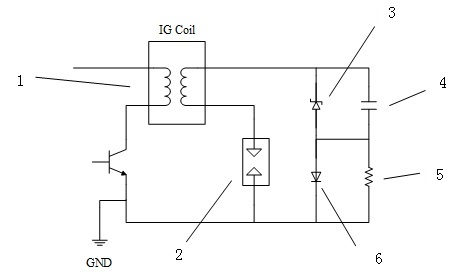
\includegraphics[width=0.8\textwidth]{thesis_figure/ion_struct}
	\caption{电容式离子电流检测电路结构}
	\label{fig:ionstruct}
\end{figure}
其中
\begin{enumerate}[1]
\item 表示点火线圈
\item 表示火花塞电极两段
\item 表示瞬态抑制二极管,防止电压过高使电路失效
\item 是电容,作为次级电路电源
\item 是检测电阻
\item 是普通二极管,用于限定检测电阻两端最大电压
\end{enumerate}
\subsection{电容式离子电流采集信号}
电容式离子电流分为三个时期:点火干扰期,火焰前锋期和火焰后期。如下图\ref{fig:ion_basic}所示是离子电流的三个时期\cite{saitzkoff1997cylinder}。
\begin{figure}[!h]
	\centering
	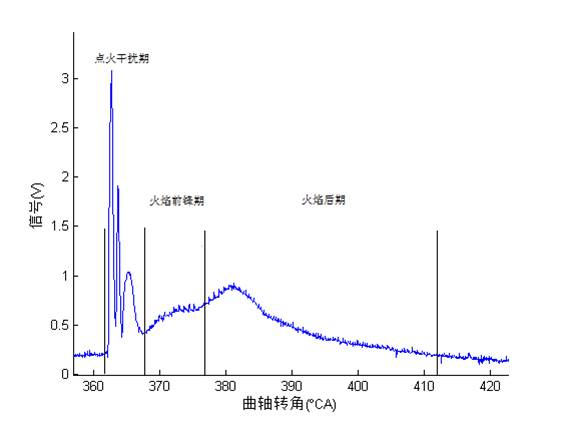
\includegraphics[width = 0.85\textwidth]{thesis_figure/model_chapter/ion_basic}
	\caption{电容式离子电流的三个时期\cite{bh2007}}
	\label{fig:ion_basic}
\end{figure}
其中点火干扰期是由点火干扰造成的。火焰前锋期由火焰锋面经过电极附近的化学电离导致的;火焰后期由火焰锋面离开电极附近后的$NO$的热电离导致的。由于点火干扰的持续时间
和点火线圈的内部结构有关系,而火焰前锋期和火焰后期和燃烧有关系,所以点火干扰期可能会和火焰前锋期甚至是火焰后期相重合。但是点火干扰的曲线和火焰前锋或火焰后期的区别在于,点火干扰
期的曲线存在稳定的震荡信号,而化学电离或热电离导致的电流频率较低。通常来说火焰后期持续到整个燃烧阶段结束。
\section{小波分析}
\subsection{小波分析理论基础}
传统的信号分析手段主要是傅里叶变换,最早来自于傅里叶于1822年发表的热传导解析理论,从那时起傅里叶变换就成为了信号处理中的主要手段。傅里叶变换的
主要思想是将时域中的信息转换为频域中的信息,通过对频域中的信息进行处理从而达到了信号处理的目的。也正因为其本质是频域信息处理,且由于频域窗口容易
产生边界效应,傅里叶变换不能够完美的解决信号处理问题。1946年Gabor提出了著名的Gabor变换,随之发展成为了短时傅里叶变换,其本质仍然是一种加窗的傅里
叶变换,随后的几十年的信号处理领域,提出了多种不同的窗口都为了克服窗口的边界效应,但是都不能够从本质上解决信号处理的问题,只能够在低频信号中采用
大时间窗,高频信号中采用小时间窗的手段不完美的解决问题。\par
自从20世纪80年代末小波分析方法提出后,揭示了频域信号和时域信号之间关系的本质,提出了著名的影响深远的小波变换。
傅里叶变换是基于正弦信号的变换,而小波变换是基于小波函数的变换,因此傅里叶变换其实是小波变换的一种特例。由于小波基函数的正交性等特点,可以在信号的低频部分有较高的频率分辨率和较低
的时间分辨率,而在高频部分具有较高的时间分辨率和较低的频率分辨率\cite{lph2011},比傅里叶变换灵活多变,是傅里叶变换的数学本质上的前进。
\par 在实际应用中,计算机只能够处理离散化的信息,因此主要采用离散小波基函数进行小波分析。以下即是连续小波序列$\psi_{a,b}(t)$和连续小波变换$W_{f}(a,b)$的离散化。
在连续小波中,考虑小波函数
\begin{equation}
	\psi_{a,b}=|a|^{-\frac{1}{2}}\psi(\frac{t-b}{a})
\end{equation}
这里$b\in R$,$a\in R_{+}$,且$a\neq0$,$\phi$是容许的,为方便起见,在离散化中,总限制$a$只取正值,这样相容性条件\cite{lyhsz2008,dys2005}就变为
\begin{equation}
	C_{\psi}=\int^{\infty}_{0}\frac{\mid \widehat{\psi}(\overline{\omega})\mid}{\mid \overline{\omega}\mid}d\overline{\omega} < \infty
\end{equation}
通常\cite{shr2009},把连续小波变换中尺度参数$a$和平移参数$b$的离散化公式分别取作$a=a_{0}^{j}$,$b=ka_{0}^{j}b_{0}$,这里$j\in Z$,扩展步长$a_{0}\neq 1$是固定值,
通常来说,总是假定$a_{0}>1$,由于$m$可以取正也可以取负,因此假定不会影响结果。所以对应的离散小波变换函数$\psi_{j,k}(t)$即可写作
\begin{equation}
	\psi_{j,k}(t)=a^{-\frac{j}{2}}_{0}\psi(\frac{t-ka_{0}^{j}b0}{a_{0}^{j}})=a_{0}^{-\frac{j}{2}}\psi(a_{0}^{-\frac{j}{2}}t-kb_{0})
\end{equation}
而离散化小波系数则可表示为
\begin{equation}
	C_{j,k}=\int_{-\infty}^{\infty}f(t)\psi_{j,k}^{*}(t)dt=<f,\psi_{j,k}>
\end{equation}
其重构公式为
\begin{equation}
	f(t)=C\sum_{-\infty}^{\infty}\sum_{-\infty}^{\infty}C_{j,k}\psi_{j,k}(t)
\end{equation}
其中$C$是一个与信号无关的常数。由此可以看到信号序列$f(t)$可以由信号无关量$C$和小波函数$\psi$组成。
\subsection{多分辨率分析}
多分辨率分析是一种分析方法,其本质作用是可以得到构造小波函数和尺度函数的双尺度方程。通过这种方法,即使在不知道小波函数和尺度函数的解析公式的情况下,仍然可以
得到离散化的小波函数和尺度函数,从而可以解决离散化的小波分析问题。
\par 设$(\{ V_{m};m\in Z\} ;\phi(t))$是一个正交多分辨率分析,则存在$\{ h_{k} \}\in l^{2}$使得下面的双尺度方程
\begin{equation}
	\phi(x) = \sum_{k}h_{k}\phi(2x-k)
\end{equation}
成立,并且利用尺度函数$\phi(x)$构造小波函数
\begin{equation}
	\psi(x)=\sum_{ki}g_{k}\phi(2x-k)
\end{equation}
其中$h_{k}=2\int_{-\infty}^{\infty}\phi(x)\overline{\phi(2x-k)}dx$,$g_{k}=(-1)^{k}\overline{h_{1-k}}$。
\par 根据上述理论多分辨率分析可以得到离散化的尺度函数和小波函数的获得方法。
\subsection{小波函数分析步骤}
小波函数分析一共分为四步\cite{2006matlab}。第一步是采样。如果待分解的是模拟信号$f(t)$,选择$N=2^{n}$,得到采样信号值$a_{k}^{n}=f(\frac{k}{2^{n}})$,其中$k$的取值保证$\frac{k}{N}$位于信号$f(t)$发生的时间范围
之内,并在每个不小于$\frac{1}{N}$的时间段内都能取到采样信号$a_{k}^{n}=f(\frac{k}{2^{n}})$,于是可以用信号
\begin{gather}
f_{n}(x)=\sum_{k\in Z}a_{k}^{n}\phi(2^{n}x-k)
\end{gather}
对连续信号$f(t)$进行高精度的近似。
\par 第二步是分解。设信号$f_{n}(x)$逐级分解为
\begin{gather}
	f_{n}(x)=W_{n-1}(x)+W_{n-2}(x)+...+W_{l-1}(x)+f_{l-1}(x) \nonumber \\
			=W_{n-1}(x)+W_{n-2}(x)+...+W_{0}(x)+f_{0}(x)
\end{gather}
\par 其中
\begin{gather*}
W_{l-1}(x)=\sum_{k\in Z}b_{k}^{l-1}\psi(2^{l-1}x-k)\\
f_{l-1}(x)=\sum_{k\in Z}a_{k}^{l-1}\psi(2^{l-1}x-k)
\end{gather*}
系数$a_{k}^{l-1}$与$b_{k}^{l-1}$按照上标
从大到小的顺序从$l=n$开始直到$l=0$结束,满足
\begin{gather}
	b_{k}^{l-1}=\frac{a_{2k}^{l}-a_{2k+1}^{l}}{2}\\
	a_{k}^{l-1}=\frac{a_{2k}^{l}+a_{2k+1}^{l}}{2}
\end{gather}
\par 第三步是信号处理。将分解后的信号表示成下面的形式
\begin{gather}
	f_{n}(x)=\sum_{l=0}^{n-1}W_{l}(x)+f_{0}(x)\nonumber \\
			=\sum_{l=0}^{n-1}(\sum_{k\in Z}b_{k}^{l}\psi(2^{l}x-k))+\sum_{k\in Z}a_{k}^{0}\phi(x-k)
\end{gather}
信号处理的过程就是根据实际情况对$b_{k}^{l}$作适当的修正。
\par 第四步是信号重构。设重构后的信号值满足
\begin{equation}
	\widetilde{f_{n}}(x)=\sum_{k\in Z}a_{k}^{n}\phi(2^{n}x-k)
\end{equation}
则上述信号值可以通过下面的递推过程得到
\begin{equation}
	\widetilde{a}^{l}=\widetilde{L}U\widetilde{a}^{l-1}+\widetilde{H}U\widetilde{b}^{l-1}, l=1,2,3,...,n
\end{equation}
其中$\widetilde{a}^{l}$和$\widetilde{b}^{l}$,$l=0,1,2,3,...,n$是根据第二、第三步得到的修正系数。\par
在所有的四步计算中,最为主要的就是第三步信号处理过程,在该过程中对小波基函数的系数进行修正就可以得到不同的结果。如
果要对信号进行去噪,则可以对高频的小波基函数的系数进行清除;如果要对信号进行压缩处理,则可以对小波基函数的系数进行阈值设
定,从而去除不必要的频率的小波基函数。
\subsection{小波分析的特点}
\begin{enumerate}[1)]
	\item~\textbf{灵活性}\quad 由于小波基函数$\phi(x)$不是唯一的,通过小波函数的构造方法就可以构造出任意的小波基函数。
	但是小波基函数的构造要和问题相结合。而傅里叶变换不能够改变其变换的基函数,灵活性受到了很大的限制。
	\item~\textbf{快速性}\quad 由尺度函数和两尺度关系来推导的小波系数,在未知小波函数的解析表达式情况下也可以对信号进行分析。
	并且在不同的频率段上可以进行细分,而傅里叶分析无法做到对特定的频率段进行细分观察。
	\item~\textbf{双域性}\quad 小波分析是时频分析,同时揭示了频域和时域两个领域的信号特征。而傅里叶变换只能在单域中显示信号特性。
	\item~\textbf{深刻性}\quad 小波理论具有很深刻的数学根基,其发展来自于数学的推导而不是像傅里叶变换更多的来自于工程应用中。
\end{enumerate}
\subsection{常见的可离散小波}
常见的可离散小波主要有db小波,sym小波,coif小波和dmey小波。其中sym小波和coif小波都是db小波的改进版本,且db小波和sym小波都有阶数选择问题。这两个
小波的阶数越大,分析得到的信号越加的平滑。不仅如此,sym小波相对于db小波具有更好的对称性,因此在信号重构方面更加的不容易失真。coif小波具有最大为五阶
的阶数,其相对于db和sym小波来说具有更好的近似对称性。由于其最高只有五次阶数且是更近似对称小波,往往比db和sym小波有更快速的计算能力。
dmey小波是离散meyer小波,由于是标准的对称小波,有快速算法,往往比前面的几个小波计算速度更快。
\subsection{离散小波之间的比较}
根据不同的应用情况,需要选取不同的小波基函数,一般的选择原则如下:
\par (1)正交性。正交性的目的在于简化工程分析,方便对数据进行处理。
\par (2)紧支性。紧支性的小波具有很好的时频局部特性,能够比较方便的用计算机语言实现。
\par (3)对称性。对称的小波基函数具有线性相位特性,这种特性有利于对图像进行分析和重构,其重构图像的边缘不容易失真。
\par (4)正则性。正则性的小波基函数对信号分析之后产生的曲线平滑,是函数频域能量的一种度量。
\par (5)消失矩。消失矩的阶数越大,越是能够对信号的高频部分进行精细分析,同时可以提高信号的衰减程度。\par
下表\ref{tab:lsxb}所示的是所有的可以进行离散小波变换的小波比较\cite{wxf2003}。\par
\begin{table}[!h]
	\centering
	\caption{可离散变换的小波函数比较}
	\label{tab:lsxb}
	\begin{tabular}{|c|c|c|c|c|}
	\hline
	小波名称&正交性&双正交性&紧支撑性&支撑长度\\\hline
	db&是&是&是&2N-1\\\hline
	sym&是&是&是&2N-1\\\hline
	dmey&是&是&是&有限长度\\\hline
	coif&是&是&是&6N-1\\\hline
	\multicolumn{5}{c}{}
	\end{tabular}
	\begin{tabular}{|c|c|c|c|c|}
	\hline
	小波名称&滤波器长度&对称性&小波函数消失矩阶数&尺度函数消失矩阵数\\\hline
	db&2N&对称&N&-\\\hline
	sym&2N&近似对称&N&-\\\hline
	dmey&[-8,8]&对称&-&-\\\hline
	coif&6N&近似对称&2N&2N-1\\\hline
	\end{tabular}
\end{table}
小波类型的选择需要针对不同的问题采取不同的处理方式。
例如对于分段多项式结构组成的信号,db小波比较适用;局部三角函数基比较合适\cite{zyclz2004}分析包含正弦分量的信号。如何
根据分析信号的特点,结合任务来优化设计小波函数一直是值得探讨的问题,迄今为止还没有系统完整的总结。且对于一些特定的离散问题,还可以通过利用多分辨率分析的方法自己构造离散的尺度函数和
小波函数。
\section{高斯曲线拟合}
\subsection{高斯函数}
高斯函数是在各个学科和工程中广泛使用的一种函数。高斯函数的形式为:
\begin{equation}
	f(x)=ae^{-\frac{(x-b)^2}{c^2}}
\end{equation}
其中$a$,$b$,$c$为实常数,且$a>0$。
\par  $c^2=2$的高斯函数是傅里叶变换的特征函数\cite{wcpyh2006}。对高斯函数进行傅里叶变化不会改变函数的本质,仍然是高斯函数。
高斯函数的不定积分是误差函数。\par
\subsection{离子电流拟合原理和方法}
Saitzkoff\cite{saitzkoff1996ionization}在缸内气体完全燃烧并且达到热化学平衡情况下推导了火焰后期的离子电流的理论公式。
\begin{equation}
	\frac{I}{I_{m}}=\frac{1}{\frac{p}{p_m}}^{\frac{1}{2}-\frac{3}{4}\frac{\gamma -1}{\gamma}}e^{-\frac{E_i}{2\kappa T_m}[\frac{1}{(\frac{p}{p_m})^{\frac{\gamma -1}{\gamma}}}-1]}
\end{equation}
其中$I$是离子电流,$I_{m}$是离子电流最大值,$p$是缸压,$p_{m}$是缸压最大值,$T_{m}$是缸内最大温度,$\gamma$是比热容比,$\kappa$是波尔兹曼常数,$E_{i}$是
离子电流能量。该公式与高斯函数相近。所以可以将火焰后期的离子电流近似拟合成高斯曲线。\par
L.Eriksson和L.Nielsen\cite{eriksson1996ignition,eriksson1997closed,eriksson1997ionization}采用该方法能够准确地估计缸压最值对应相位,从而可以
自适应调整点火提前角,提高了发动机的燃烧效率。Magnus Hellring等人也通过了拟合曲线的方法控制了缸压峰值相位的位置\cite{hellring2001comparison}。\par
而由于排气过程不能将缸内的所有废气排除缸内,断油循环和断火循环中仍然存在部分带$NO$离子
的废气,仍然可以检测到离子电流。同样道理,在正常循环的点火之前由于存在部分废气,离子电流检测电路可以检测到轻微的离子电流信号。这部分废气导致的离子电流信号也可以用高斯函数近似分析。
由此整个检测到的离子电流信号可以用两个高斯曲线拟合来进行分析。






\chapter{发动机试验台架}
\section{实验台架}
本实验台架由发动机,发动机支架,发动机附件和其他测试设备组成,其台架系统示意图如\ref{fig:platformintro}图所示。\par
\begin{figure}[!h]
	\centering
	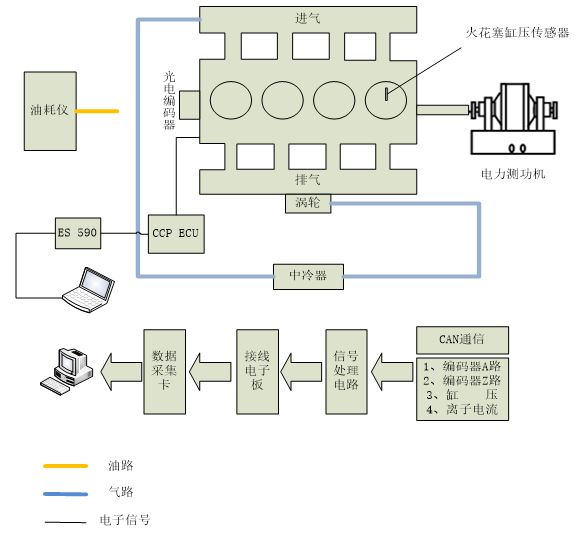
\includegraphics[width=0.85\textwidth]{thesis_figure/platformer_chapter/platformer_intro}
	\caption{台架系统示意图}
	\label{fig:platformintro}
\end{figure}
其中发动机是1.8T涡轮增压多点进气道喷射发动机,电力测功机为凯迈测功机,油耗仪为AVL油耗仪,通过Kistler火花塞式缸压传感器来测量缸压,用光电编码器
来同步信号并确定曲轴上止点位置。通过改造普通的点火线圈将二级线圈高压点和接地点接入离子电流采集电路中来采集离子电流信号。
\subsection{发动机}
发动机实物图如\ref{fig:ecu}所示,该发动机是一台四冲程PFI涡轮增压发动机,缸径为\SI{86}{\mm},行程为\SI{77.4}{\mm},
排量为\SI{1.798}{L},最大功率为\SI{130}{\kW},最大转矩为\SI{230}{\N\m}。
其ECU为联合汽车电子有限公司提供的基于ME788控制系统的ECU,实物图如图\ref{fig:ice}所示。\par
\begin{figure}[!ht]
	\begin{minipage}[h]{0.5\linewidth}
		\centering
		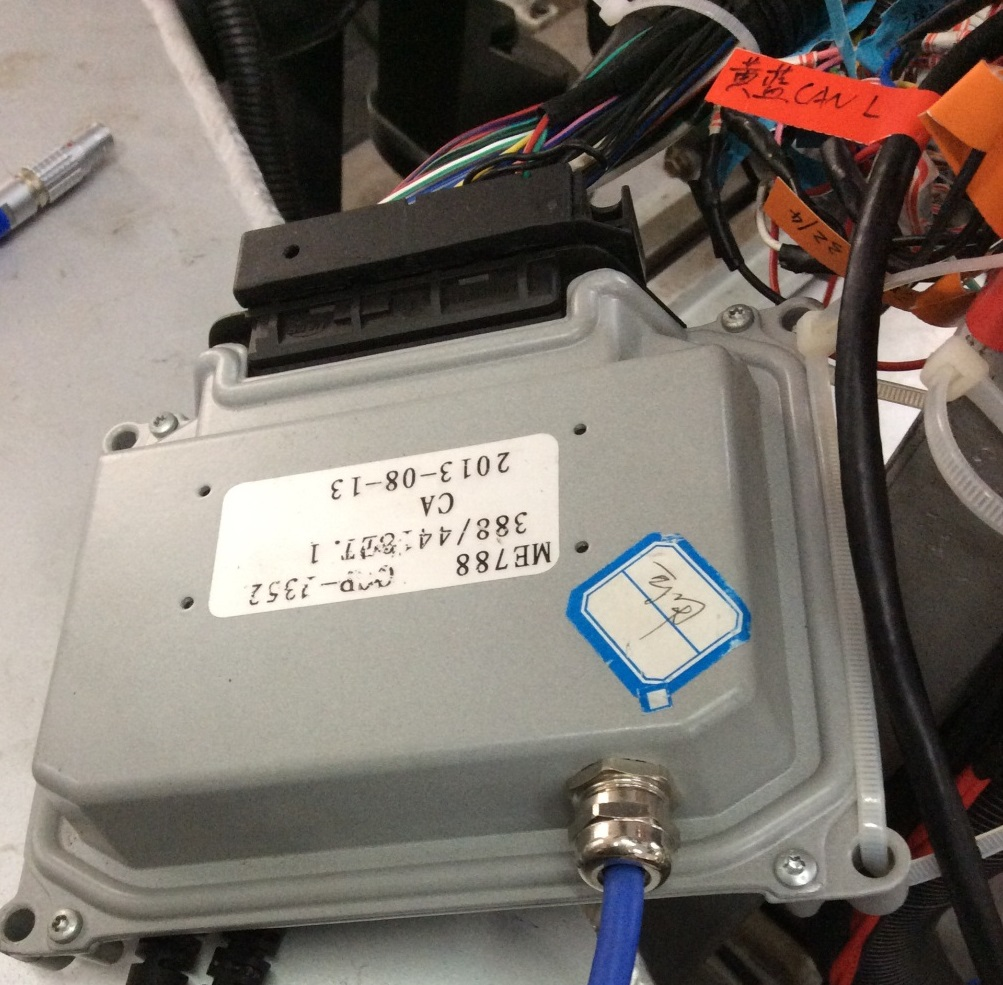
\includegraphics[height=5cm]{thesis_figure/platformer_chapter/ecu}
		\caption{ECU实物图}
		\label{fig:ecu}
	\end{minipage}
	\begin{minipage}[h]{0.5\linewidth}
		\centering
		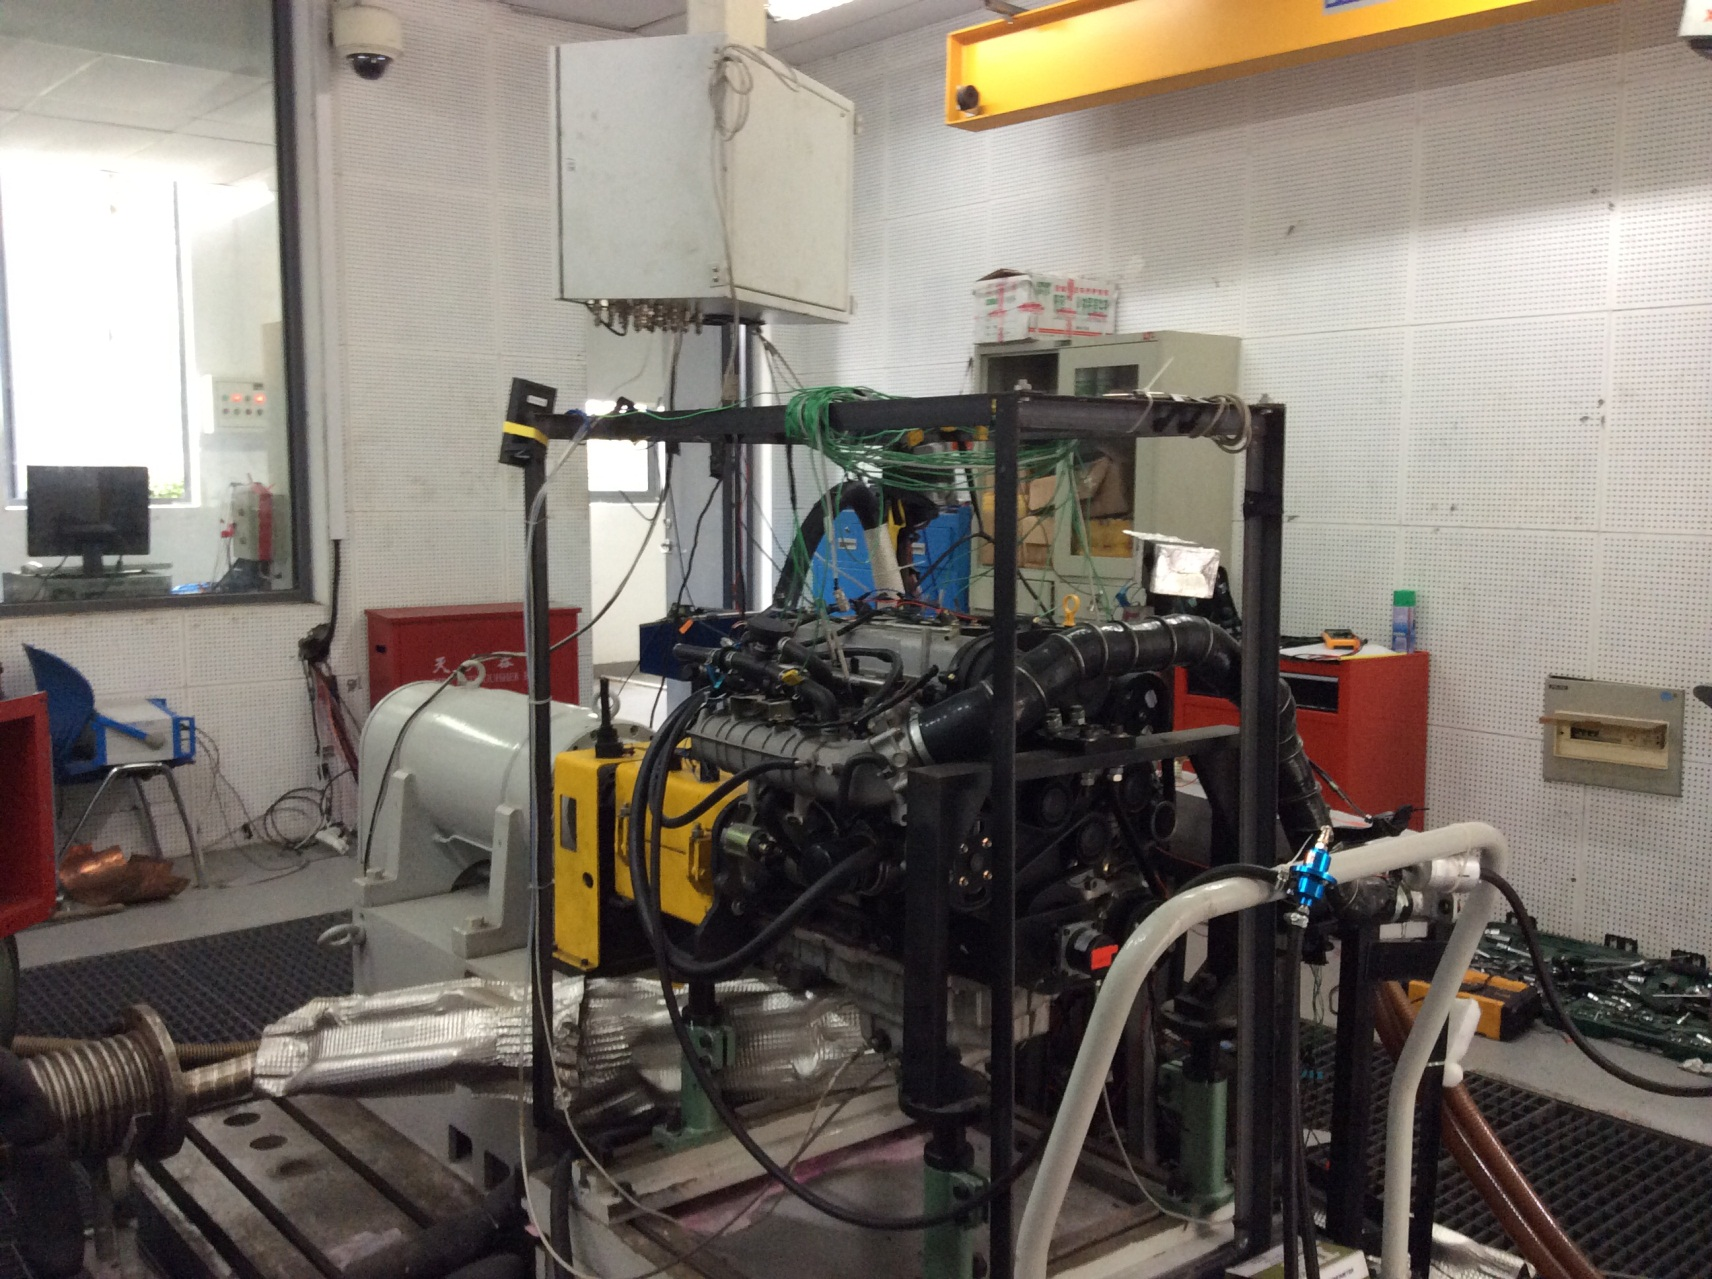
\includegraphics[height=5cm]{thesis_figure/platformer_chapter/ice}
		\caption{发动机实物图}
		\label{fig:ice}
	\end{minipage}
\end{figure}
ECU一端连接发动机线束,另一端通过CAN线连接到上位机。在上位机上安装INCA等软件,通过INCA等软件将该ECU的数据显示并保存出来,用MDA对保存的数据进行简单的数据分析。\par
除此之外,发动机靠近测功机的缸内安装缸压传感器,缸压传感器通过采集卡将数据保存到上位机中。由此,发动机的各项参数可以分别通过ECU和采集卡分别保存到上位机中,通过
采集频率的设定和算法的开发保证分别采集的数据具有相同的采集频率,以便进行后续处理。
\subsection{测功机}
交流电力测功机是目前市场上最先进的动力加载测试设备,在动力机械低速及高速的加载测功实验中都有非常出色的表现,可靠性较高同时又便于维护。
本次实验采用的交流电力测功机系统来自凯迈(洛阳)机电有限公司,该系统基于变频技术开发,精度和稳定性较高,结构简单便于维护,便于进行自动化操作
,形成了一个系列产品。如图\ref{fig:dlcgj}是测功机安装布线的示意图。
\begin{figure}[htb]
	\centering
	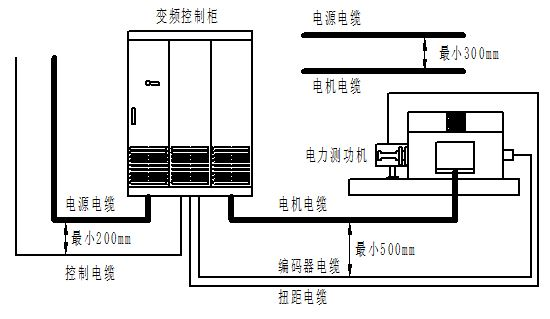
\includegraphics[width=0.75\textwidth]{thesis_figure/platformer_chapter/dlcgj}
	\caption{DCW系列交流电力测功机系统安装布线示意图}
	\label{fig:dlcgj}
\end{figure}
\par 该交流电力测功机主要由三相异步交流电机、可四象限运行的交流调速柜、控制系统、采集系统组成。交流变频调速柜分为整流
单元和逆变单元两部分组成。整流单元可以将380V交流电转换为内部流点,再经过变频成为交流电输出到三相异步电机中。
\begin{figure}[htb]
	\centering
	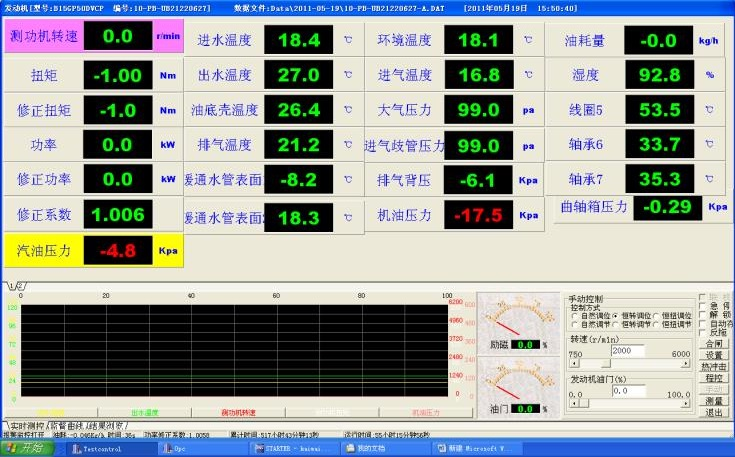
\includegraphics[width=0.75\textwidth]{thesis_figure/platformer_chapter/cgjkzjm}
	\caption{测功机控制界面}
	\label{fig:cgjkzjm}
\end{figure}
\par 测功机的实物图如\ref{fig:dlcgjswt}所示。
测功机通过改变交流电的频率和电压来对测功机的转速进行控制。通过电机四象限转换,将电极交流电转变为工业用电标准的交流电,传到电网,同时可以达到
加载转矩的目的。测功机控制界面如图\ref{fig:cgjkzjm}所示,该界面实时显示台架试验过程中转速、水温、扭矩等状态参数,并具有急停功能。\par
\begin{figure}[htb]
	\centering
	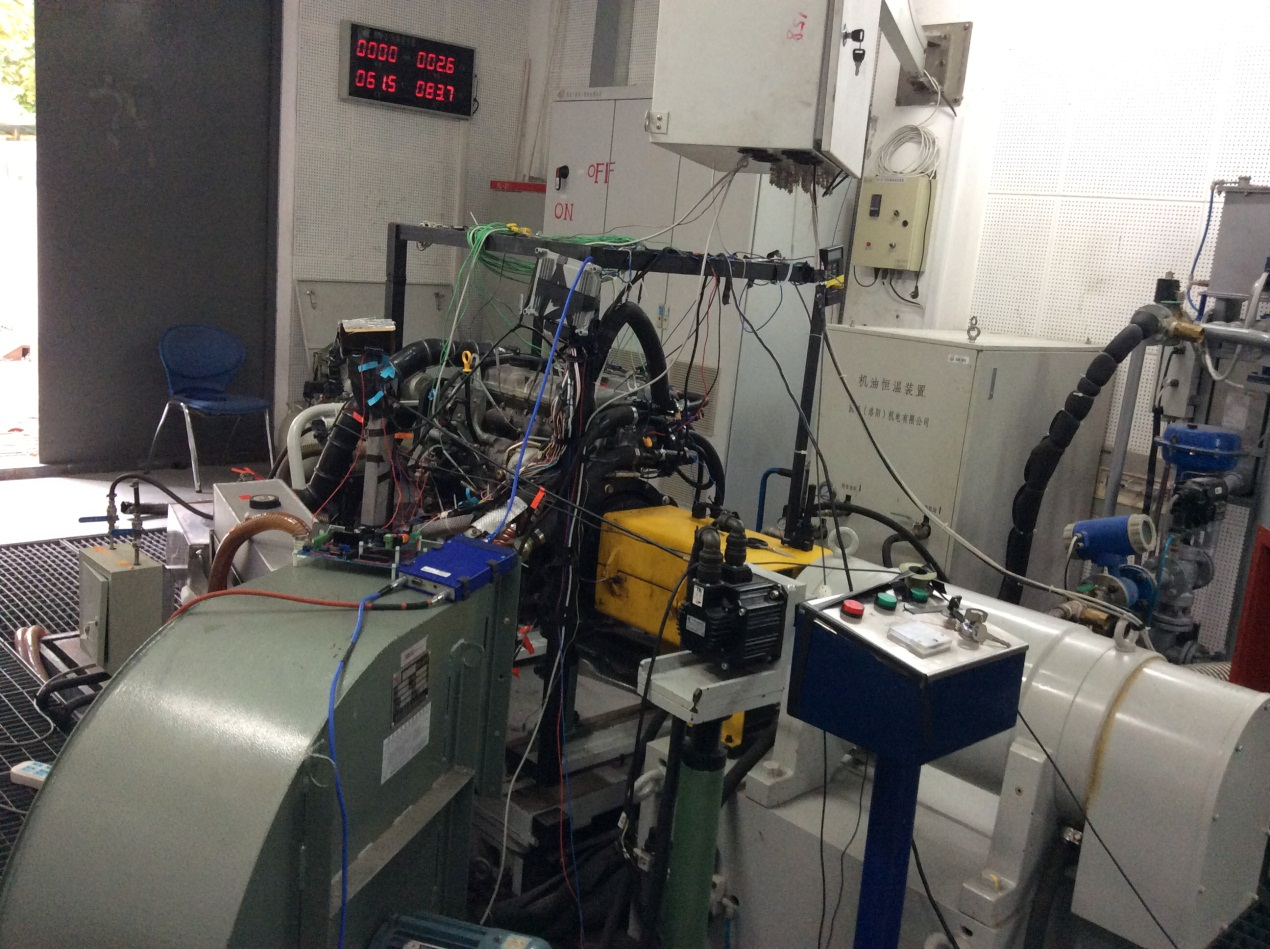
\includegraphics[width=0.75\textwidth]{thesis_figure/platformer_chapter/dlcgjswt}
	\caption{电力测功机实物图}
	\label{fig:dlcgjswt}
\end{figure}
电力测功机的参数如表\ref{tab:dlcgjjtcs}所示,总体来看该测功机性能优秀,适合本实验的进展。
\begin{table}[H] 
 	\centering 
 	\caption{电力测功机具体参数} 
 	\label{tab:dlcgjjtcs} 
 	\begin{tabular}{|c|c|c|} 
 	\hline 
 	测量参数 & 测量范围 & 精度\\\hline 
 	转速 & $0\thicksim10000\si{r/min}$ &$\pm 1\si{r/min}$ \\\hline 
 	扭矩 & $0\thicksim500N\centerdot m$ &$\pm 0.4\%\si{FS}$ \\\hline 
 	燃油消耗 &$0\thicksim100\si{Kg\per h}$ & $\pm 0.12\%\si{FS}$ \\\hline 
 	环境温度 &$0\thicksim50^{\circ}C$ & $\pm 0.5\%\si{FS}$ \\\hline 
 	环境湿度 &$0\thicksim100\%$ & $\pm 2\% RH$ \\\hline 
 	冷却水进温 &$0\thicksim150^{\circ}C$ & $\pm 0.5^{\circ}C$ \\\hline 
 	冷却水出温 &$0\thicksim150^{\circ}C$ & $\pm 0.5^{\circ}C$ \\\hline 
 	机油温度 &$0\thicksim150^{\circ}C$ & $\pm 0.5^{\circ}C$ \\\hline 
 	燃油温度 &$0\thicksim150^{\circ}C$ & $\pm 0.5^{\circ}C$ \\\hline 
 	中冷前温度 &$0\thicksim150^{\circ}C$ & $\pm 0.5^{\circ}C$ \\\hline 
 	中冷后温度 &$0\thicksim250^{\circ}C$ & $\pm 0.5^{\circ}C$ \\\hline 
 	排气温度 &$0\thicksim150^{\circ}C$ & $\pm 0.5^{\circ}C$ \\\hline 
 	机油压力 &$0\thicksim1000\si{KPa}$ & $\pm 0.5\%\si{FS}$ \\\hline 
 	燃油压力 &$0\thicksim1000\si{KPa}$ & $\pm 0.5\%\si{FS}$ \\\hline 
 	进水压力 &$0\thicksim600\si{KPa}$ & $\pm 0.5\%\si{FS}$ \\\hline 
 	出水压力 &$0\thicksim600\si{KPa}$ & $\pm 0.5\%\si{FS}$ \\\hline 
 	曲轴箱压力 &$-20\thicksim20\si{KPa}$ & $\pm 0.25\%\si{FS}$ \\\hline 
 	排气背压 &$0\thicksim50\si{KPa}$ & $\pm 0.5\%\si{FS}$ \\\hline 
 	中冷前压力 &$0\thicksim300\si{KPa}$ & $\pm 0.5\%\si{FS}$ \\\hline 
 	中冷后压力 &$0\thicksim300\si{KPa}$ & $\pm 0.5\%\si{FS}$ \\\hline 
 	大气压力 &$80\thicksim110\si{KPa}$ & $\pm 0.25\%\si{FS}$ \\\hline 
 	\end{tabular} 
\end{table} 
\subsection{发动机附件}
发动机附件包括增压中冷系统、冷却系统、进排气系统等。
增压中冷系统由中冷器、进气、出气、进水、出水、增压压力温度传感器等部分组成。
冷却系统分为水冷和风冷两部分,水冷由外接的冷却循环系统构成。风冷则主要是使用大功
率的风机吹排气管,实现快速降温,使温度在需要范围之内。
进气系统由自制空气滤清器和原机进气管组成,排气系统由原机排气歧管、排气管加上自制一段排气管通往实验室排气系统中,
其中,排气管上装有排气温度传感器。
\section{实验设备及器材}
\subsection{缸压传感器}
缸压传感器采用的是KISTLER提供的6118B型火花塞缸压传感器,具有3mm可换电缆,无需另外打孔即可实现缸压的测量。
它装有世界上最小的压电式高温缸压传感器。安装时,前端与燃烧室内部平齐,固有频率高于100kHz。因此,也可用
于高速发动机和爆震控制测试。其实物图和技术参数见图\ref{fig:gycgq}和表\ref{tab:gycgq}。
\begin{table}[H] 
 	\caption{缸压传感器具体参数} 
 	\label{tab:gycgq} 
 	\centering 
 	\begin{tabular}{|c|c|c|} 
 	\hline 
 	物理量 & 单位& 数值 \\ 
 	\hline 
 	重量 & g& 50\\\hline 
 	压力范围 & bar & $0\thicksim 200$ \\\hline
 	标定区间(在200$^{\circ}C$) &bar & $0\thicksim 150$ \\\hline 
 	过载 & bar & 250 \\\hline 
 	灵敏度(200$^{\circ}C$) & pC/bar & $\thickapprox10$ \\\hline 
 	固有频率 & kHz & $>100$ \\\hline 
 	室温线性度 & \%FSO & $\leq \pm$ 0.5 \\\hline 
 	加速的灵敏度(轴向和径向) & bar/g & $<0.005$ \\\hline 
 	传感器工作温度范围 & $^{\circ}C$ & $-20\thicksim 350$ \\\hline 
 	电缆工作温度范围 & $^{\circ}C$ & $-20 \thicksim 200$ \\\hline 
 	灵敏度变化($200\pm 50^{\circ}C$)&\%& $\leq\pm 1$ \\\hline 
 	短期飘移$\triangle p$ & bar & $\leq \pm 0.6$ \\\hline 
 	$\triangle p_{min}$ & \% & $\leq \pm 3$ \\\hline 
 	$\triangle p_{max}$ & \% & $\leq \pm 1.5$ \\\hline 
 	20$^{\circ}C$时传感器绝缘阻抗 & $\Omega$ & $>1013$ \\\hline 
 	200$^{\circ}C$时传感器绝缘阻抗 & $\Omega$ & $>1011$ \\\hline 
 	火花塞阻抗(1000V,室温下) & $\Omega$& $>100$ \\\hline 
 	绝缘强度 & kV& $<35$ \\\hline 
 	传感器电容 & pF/m& 110\\ 
 	\hline 
 	\end{tabular} 
\end{table}
其还配备了装有数字式双
通道电荷放大器模块的信号调理平台,通过将放大后的气缸压力信号传
给工控机采集卡记录缸内燃烧压力数据。\par
\begin{figure}[htb]
	\begin{minipage}[t]{0.5\linewidth}
		\centering
		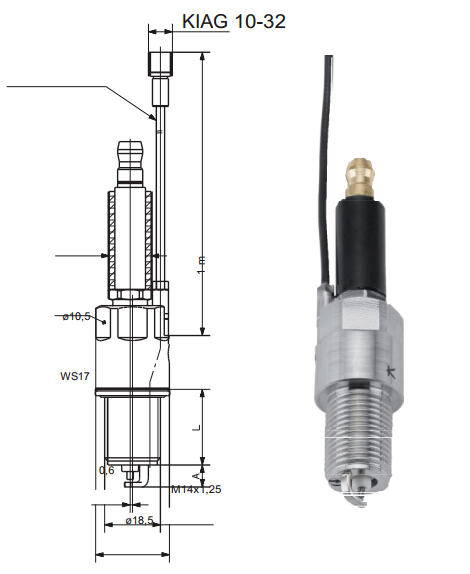
\includegraphics[width=0.8\textwidth]{thesis_figure/platformer_chapter/gycgq}
		\caption{火花塞式缸压传感器}
		\label{fig:gycgq}
	\end{minipage}
	\begin{minipage}[t]{0.5\linewidth}
		\centering
		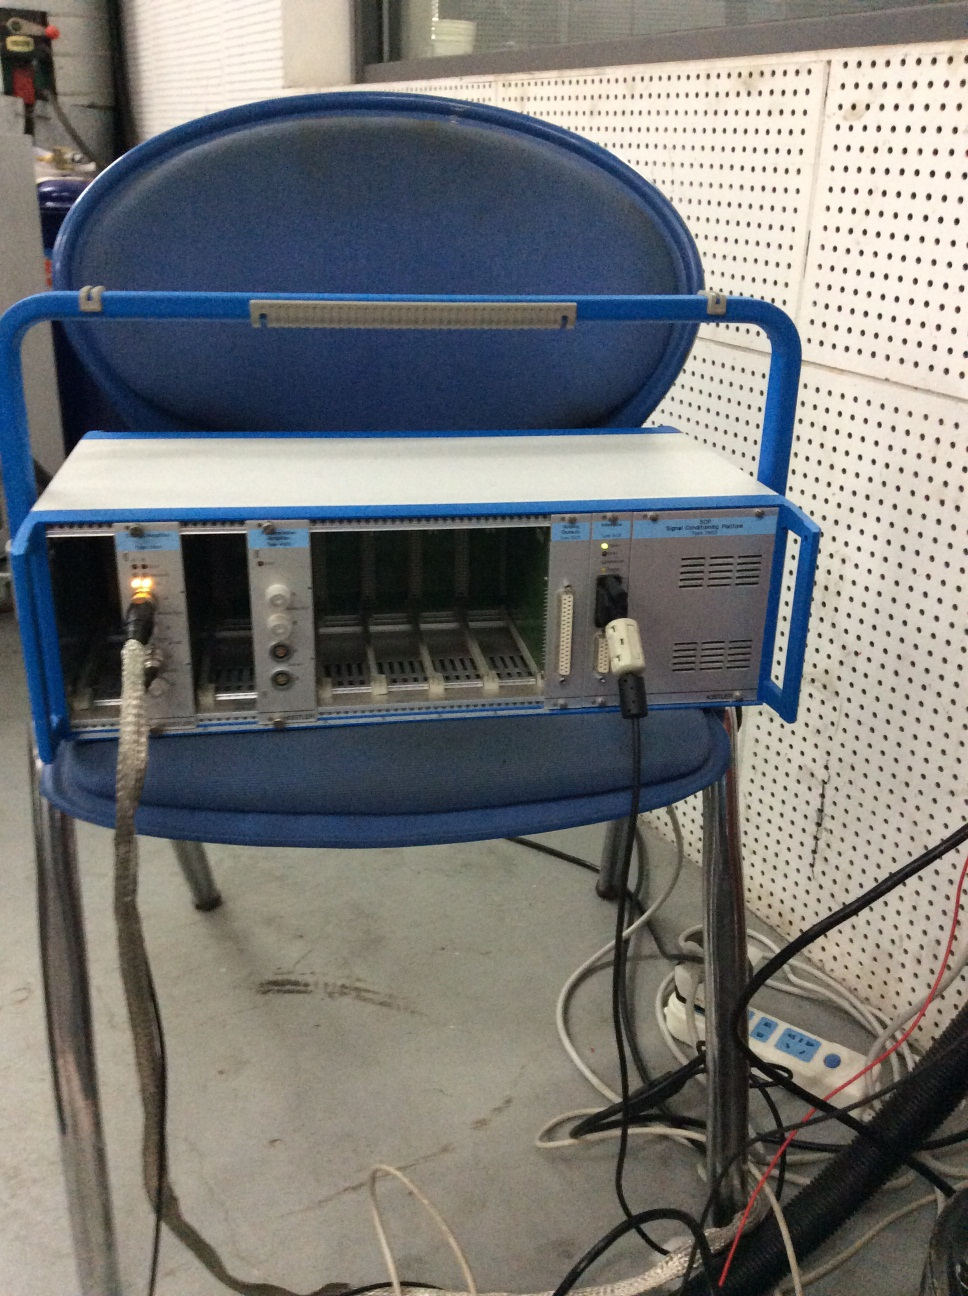
\includegraphics[width=0.8\textwidth]{thesis_figure/platformer_chapter/gycgqdhfdq}
		\caption{缸压传感器电荷放大器}
		\label{fig:gycgqdhfdq}
	\end{minipage}
\end{figure}
这种电荷放大器可以用于实验室通过压电测力仪测量力和扭矩。通过负载作用在压电传感器上产生一个正比例变化的电荷。这
个电荷信号放大器转换成比例的输出电压。电荷放大器的实物图如图\ref{fig:gycgqdhfdq}所示。
\subsection{光电编码器}
发动机正时链条侧曲轴端安装HGAIN公司的F5809型增量式光电编码器,曲轴信号测量范围720 pulse/r,测量精度$0.5^{\circ}CA$,如
图\ref{fig:gdbmq}所示。该编码器内部采用ASIC器件,具有寿命长,可靠性高,信号分辨率高,抗干扰能力较强,信号传输距离较长等优点,为
采集卡提供采样中断保证。其A路与Z路信号用于高速采集系统触发源以及作为后期数据处理的曲轴时刻参考依据。
\begin{figure}[ht]
	\begin{minipage}[H]{0.5\linewidth}
		\centering
		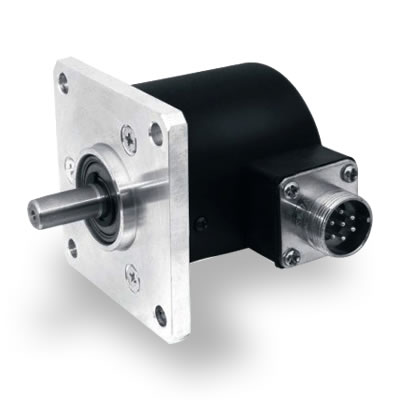
\includegraphics[width=0.8\textwidth]{thesis_figure/platformer_chapter/gdbmq}
		\caption{光电编码器}
		\label{fig:gdbmq}
	\end{minipage}
	\begin{minipage}[H]{0.5\linewidth}
		\centering
		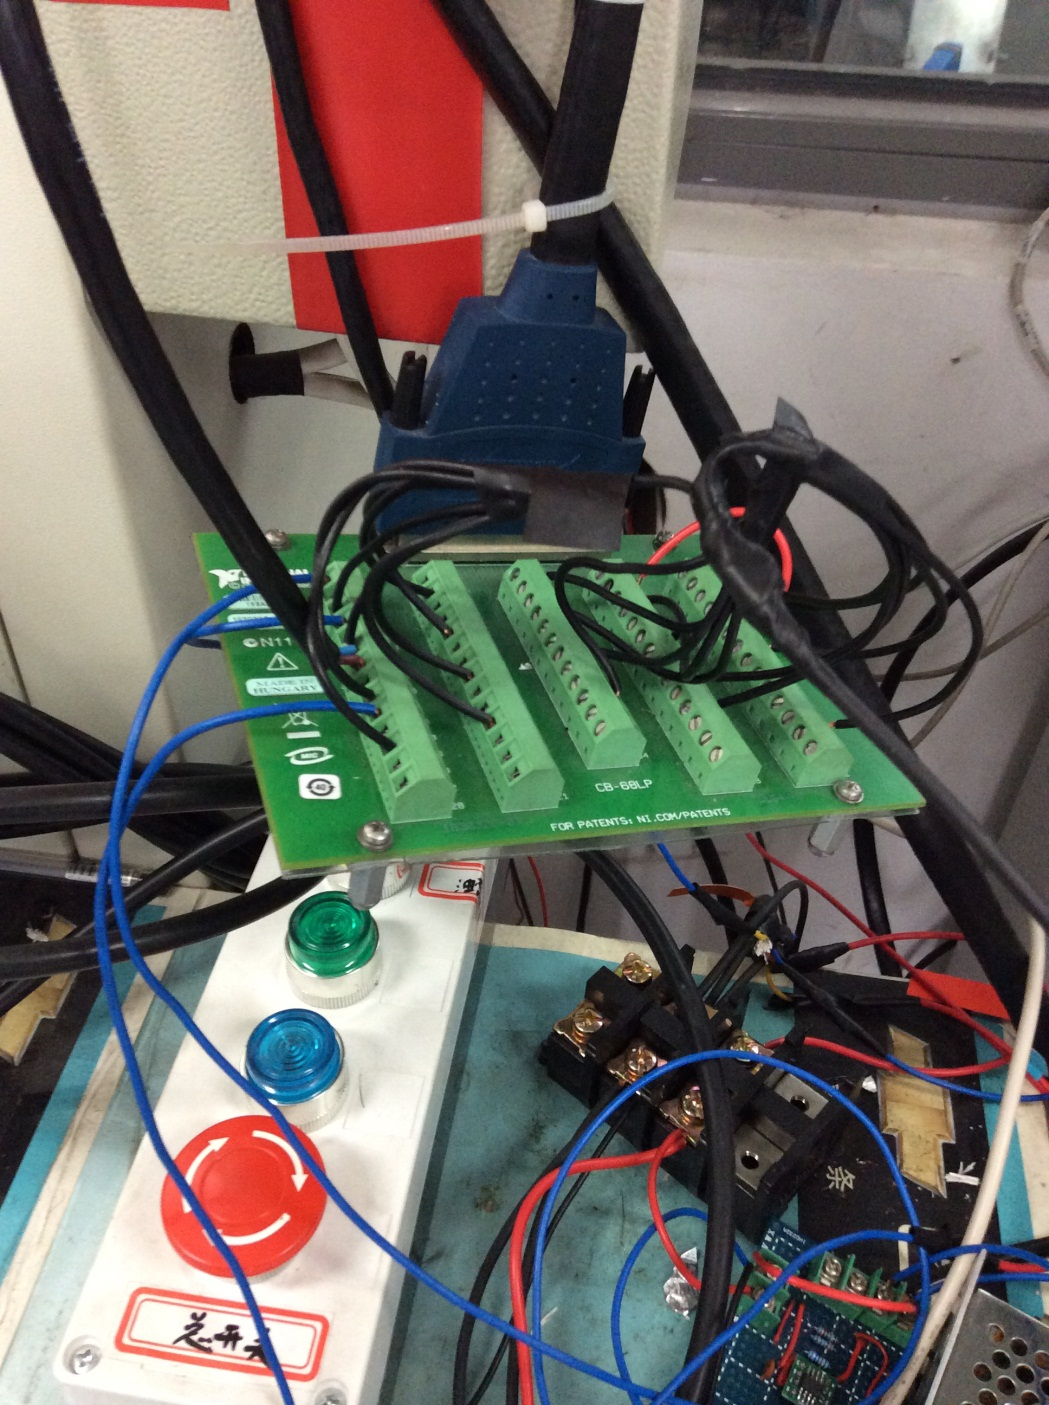
\includegraphics[width=0.8\textwidth]{thesis_figure/platformer_chapter/nicjk}
		\caption{NI公司提供的采集卡}
		\label{fig:nicjk}
	\end{minipage}
\end{figure}
\subsection{采集卡}
数据采集系统可以用来记录发动机运行过程中的各种性能参数。本试验采用NI公司的PCI 6250高速采集卡,其具备16路模拟信号输入,16
位转换精度,多通道采样频率1MHz,单通道模式下1.25MHz,最大采集幅值范围为±10V等强大功能。\par 研究离子电流特性需要采集的参数
分为两大类:第一类是缸内燃烧压力信号、离子电流信号及用于判断曲轴相位的A路和Z路信号等信号,这些信号可以表征发动机的性能和排放;
二是发动机转速、发动机负荷、爆震积分值、进气温度、进气压力、冷却水温度以及机油压力等信号,这些信号主要来自ECU的计算,并通过CAN总线传到高速采集卡中采集下来。该采
集卡能够满足以上两类需求。采集卡实物图如图\ref{fig:nicjk}所示,吊在空中是为了隔离干扰。
\subsection{采集程序}
采集程序是由Labview所编写,主要分为手动采集和触发采集两种类型,可通过记录模式进行切换。其中手动采集模式通过点击“开始”进行数据采
集,而触发采集可以设置触发条件,本文设置的是缸压值$>$阀值,采集程序会将超过该阀值的前后一段时间的数据采集下来,图\ref{fig:cjcxjm}是采集程序的界面。
\begin{figure}[htb]
	\centering
	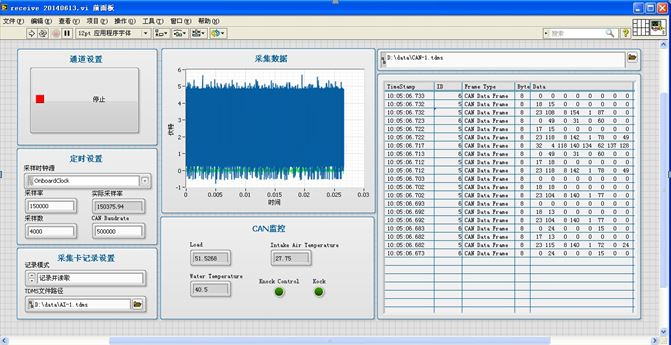
\includegraphics[width=0.85\textwidth,trim=0.25cm 0.5cm 4.5cm 1.25cm,clip]{thesis_figure/platformer_chapter/cjcxjm}
	\caption{采集程序界面}
	\label{fig:cjcxjm}
\end{figure}
\par 该采集程序主要由定时设置,采集卡记录设置,CAN监控,数据实时显示和通道开关几个部分组成。定时设置可以设置采样时钟、采样数、采样率等关键参数;采集卡记录设置
可以设置文件保存的路径,CAN监控可以实时监测采集过程是否有异常,同时也可以通过数据实时显示监控面板来查看数据采集过程是否有异常。






\chapter{离子电流干扰去除分析方法}
\section{电容式离子电流检测电路的局限性}
如下图所示的是1250r/min,2000r/min,3000r/min下在30\%,40\%,50\%时的缸压和离子电流曲线。\par
\begin{figure}[H]
	\centering
	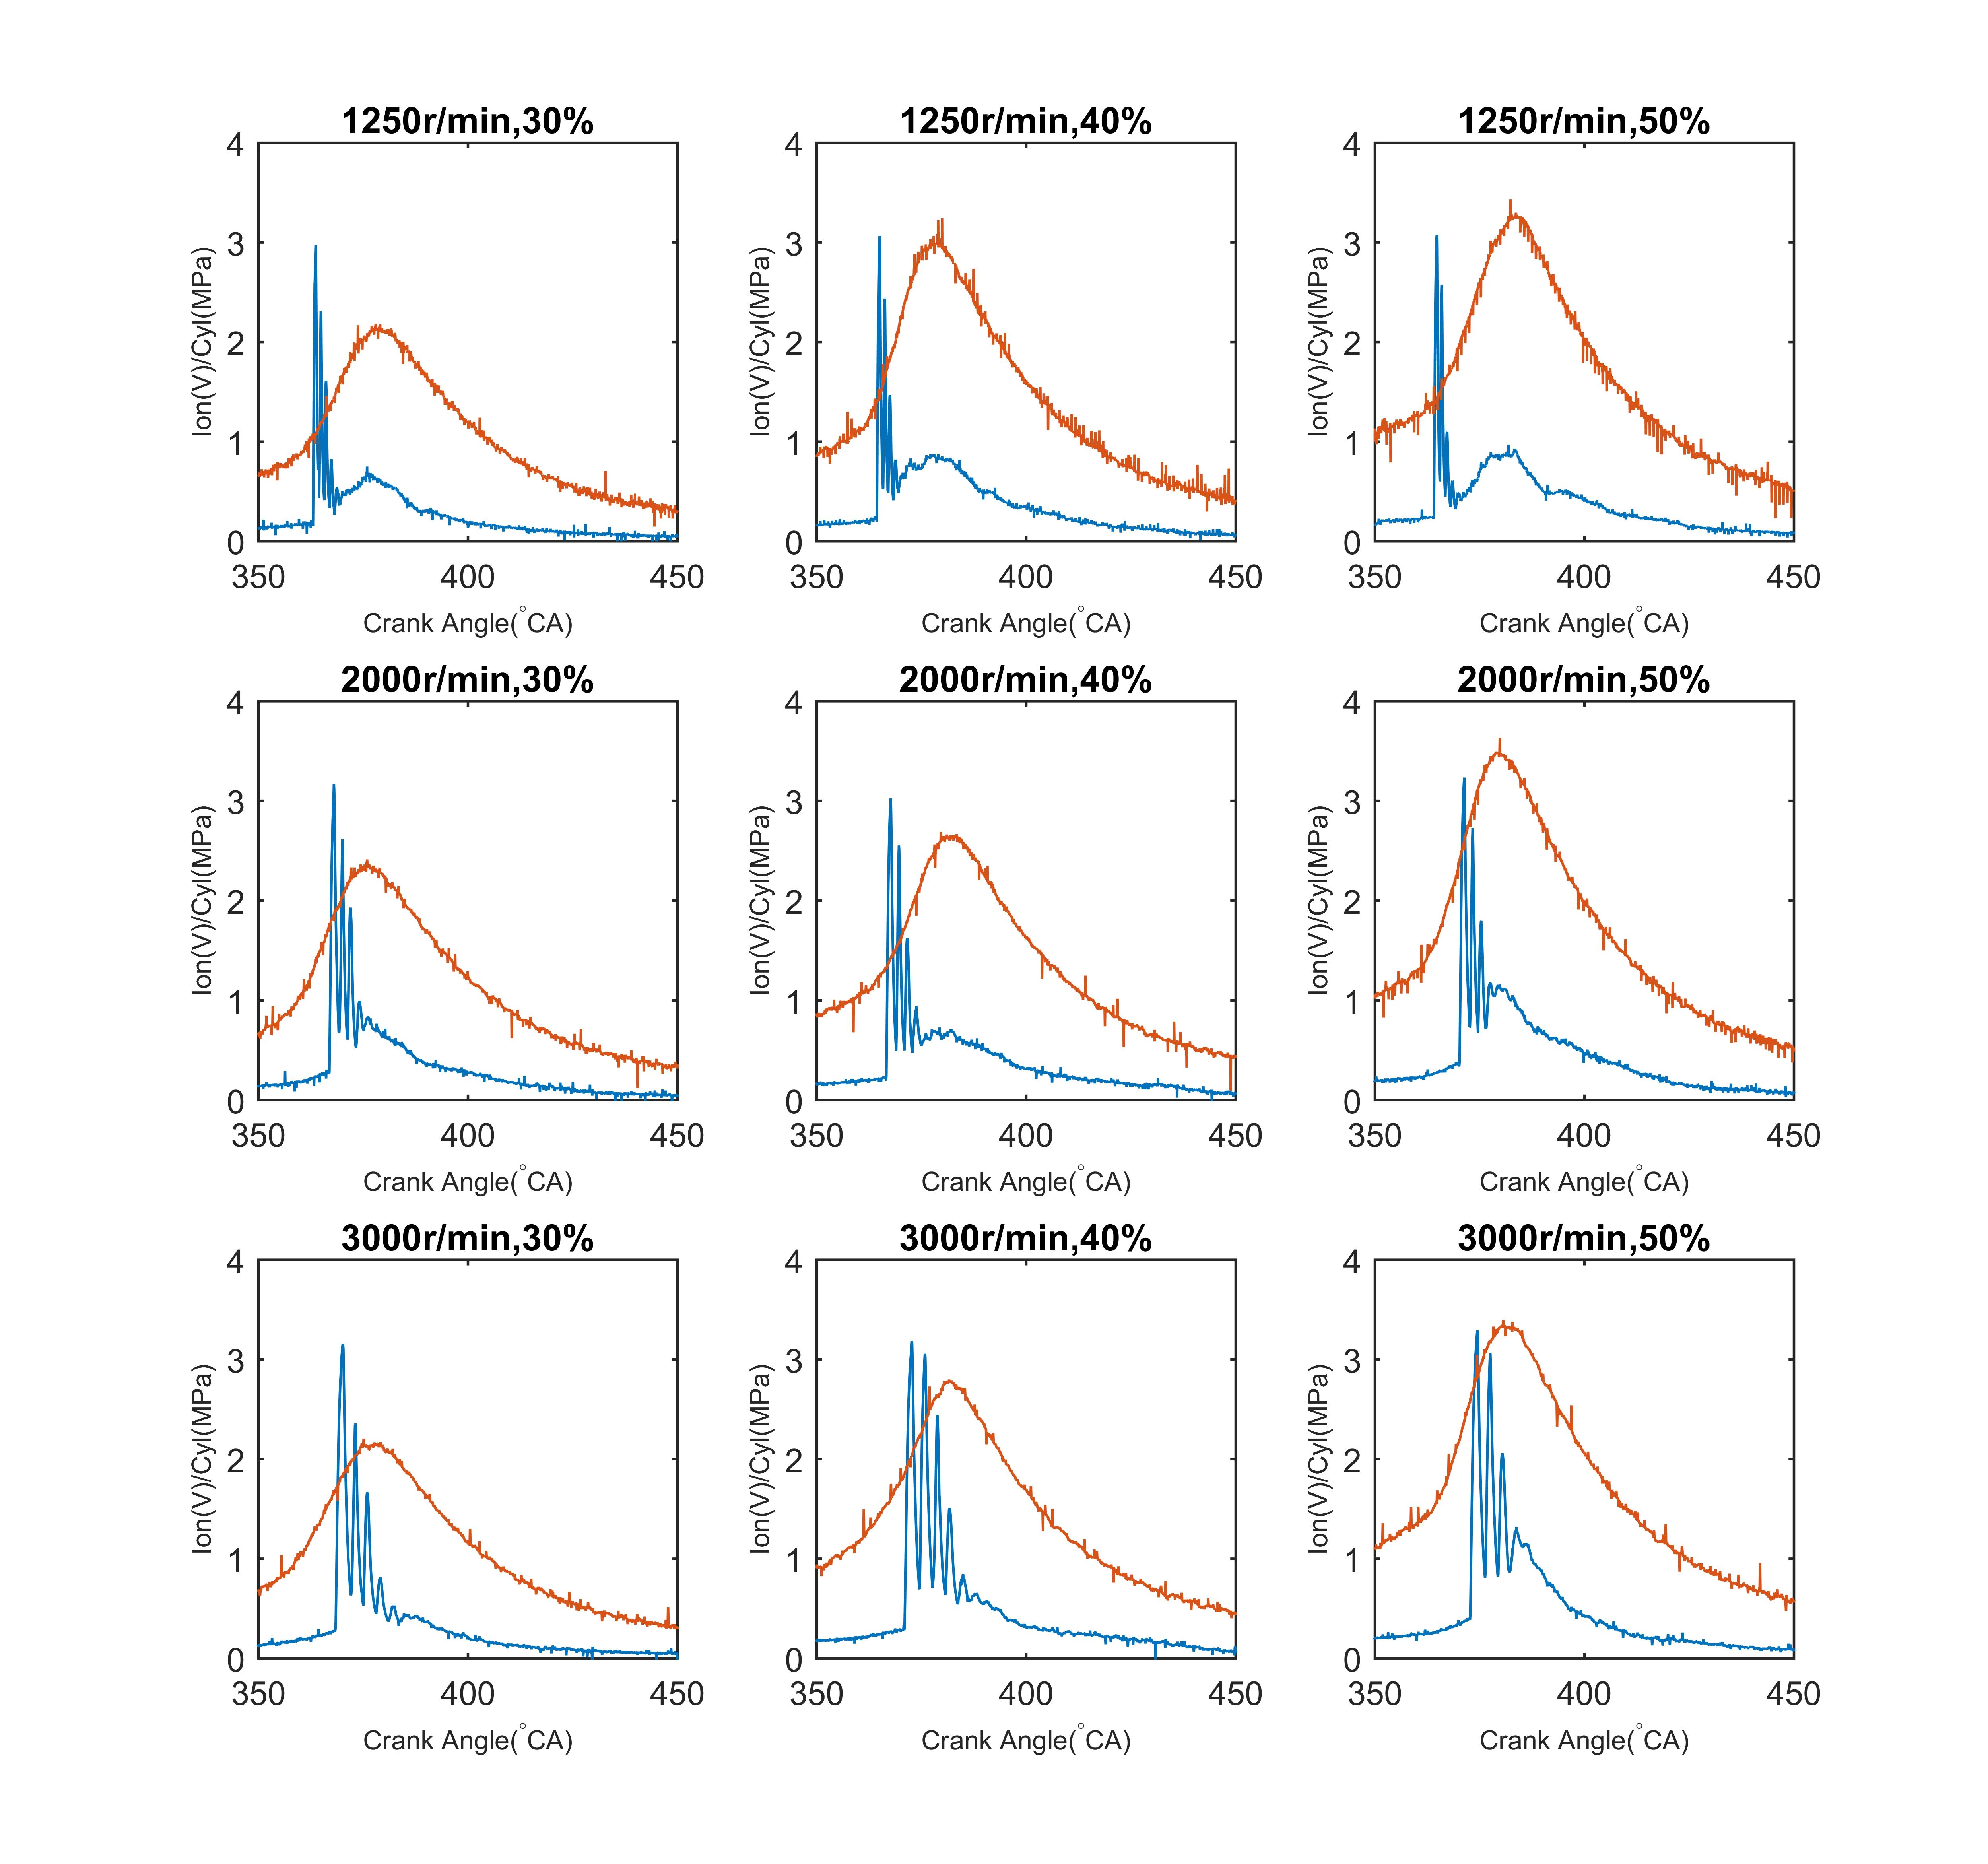
\includegraphics[width=\textwidth]{thesis_figure/ion_chapter/ion_vary_trending}
	\caption{不同转速、不同负荷下的缸压和离子电流}
	\label{fig:ion_cyp}
\end{figure}
从图\ref{fig:ion_cyp}中可以看到从上到下看是同一负荷下,随着转速增加的离子电流曲线;从左向右是同一转速下,随着负荷增大的离子电流曲线。
随着转速的增加,火焰后期的离子电流是逐渐被淹没的。也就是说点火干扰期将离子电流的性质淹没了,无法获得离子电流的特征值。
\subsection{点火放电干扰的来源和性质}
由于点火干扰期将离子电流的性质淹没,因此我们需要了解点火放电干扰的来源及其稳定的性质。如图\ref{fig:itf_rs}所示,通过检测次级电压来和离子电流进行对比可以发现,次级电压
点火放电过程的放电干扰期和离子电流的点火干扰期重合。\par
\begin{figure}[H]
	\centering
	\includegraphics[width = 0.9\textwidth]{thesis_figure/ion_chapter/interfere_comparison}
	\caption{\label{fig:itf_rs}次级电压和离子电流对比}
\end{figure}
我们将重叠的部分进行放大,可以看到两者的频率也是相同的。
经过计算可以得到该放电周期为$0.12ms$,时长为$1ms$。由以上两张图的分析结果可以知道,离子电流的点火干扰期是由次级线圈的点火放电信号导致的,会产生一个特定频率的震荡信号。我们将不同转速下的离子电流
曲线放在一起比较,可以看到如图\ref{fig:4_3_dif_rpm_ion}所示的图形。\par
\begin{figure}[!ht]
	\centering
	\includegraphics[width=0.9\textwidth]{thesis_figure/ion_chapter/4_3_dif_rpm_ion}
	\caption{不同转速下的离子电流按曲轴转角对比和按时间对比}
	\label{fig:4_3_dif_rpm_ion}
\end{figure}
左列的三张图从上到下为随着转速增加,离子电流按照曲轴转角进行对比,曲轴转角窗口长度为100度,可以发现点火震荡信号在不断淹没火焰前锋期和火焰后期。右列的三张图从上到下为随着转速增加,
离子电流按时间进行对比,时间窗口长度为5毫秒时间,可以发现震荡信号的频率和长度不变。左右两列曲线分别对应了该工况下的同一个循环,由此可以知道该震荡信号具有稳定的时间长度,稳定的频率特性。
\subsection{断油情况下的点火干扰分析}
当发动机断油情况下,点火线圈仍然进行点火过程,但是缸内由于没有燃气,无法形成化学电离过程的离子电流信号,所以断油情况下的点火干扰具有稳定而且清晰的特征。如图\ref{fig:dy_ion}所示是一个断油情况下的电容
式检测电路检测到的电压曲线。
\par 从图\ref{fig:dy_ion}中可以看到缸压曲线峰值相位在上止点360度位置,说明该循环处于纯压缩循环。可以看到此时的离子电流信号的峰值位置也是上止点位置,此时的离子电流信号是热电离导致的,没有化学电离产生的离子电流信号。
\begin{figure}[H]
\begin{minipage}[t]{0.5\linewidth}
	\centering
	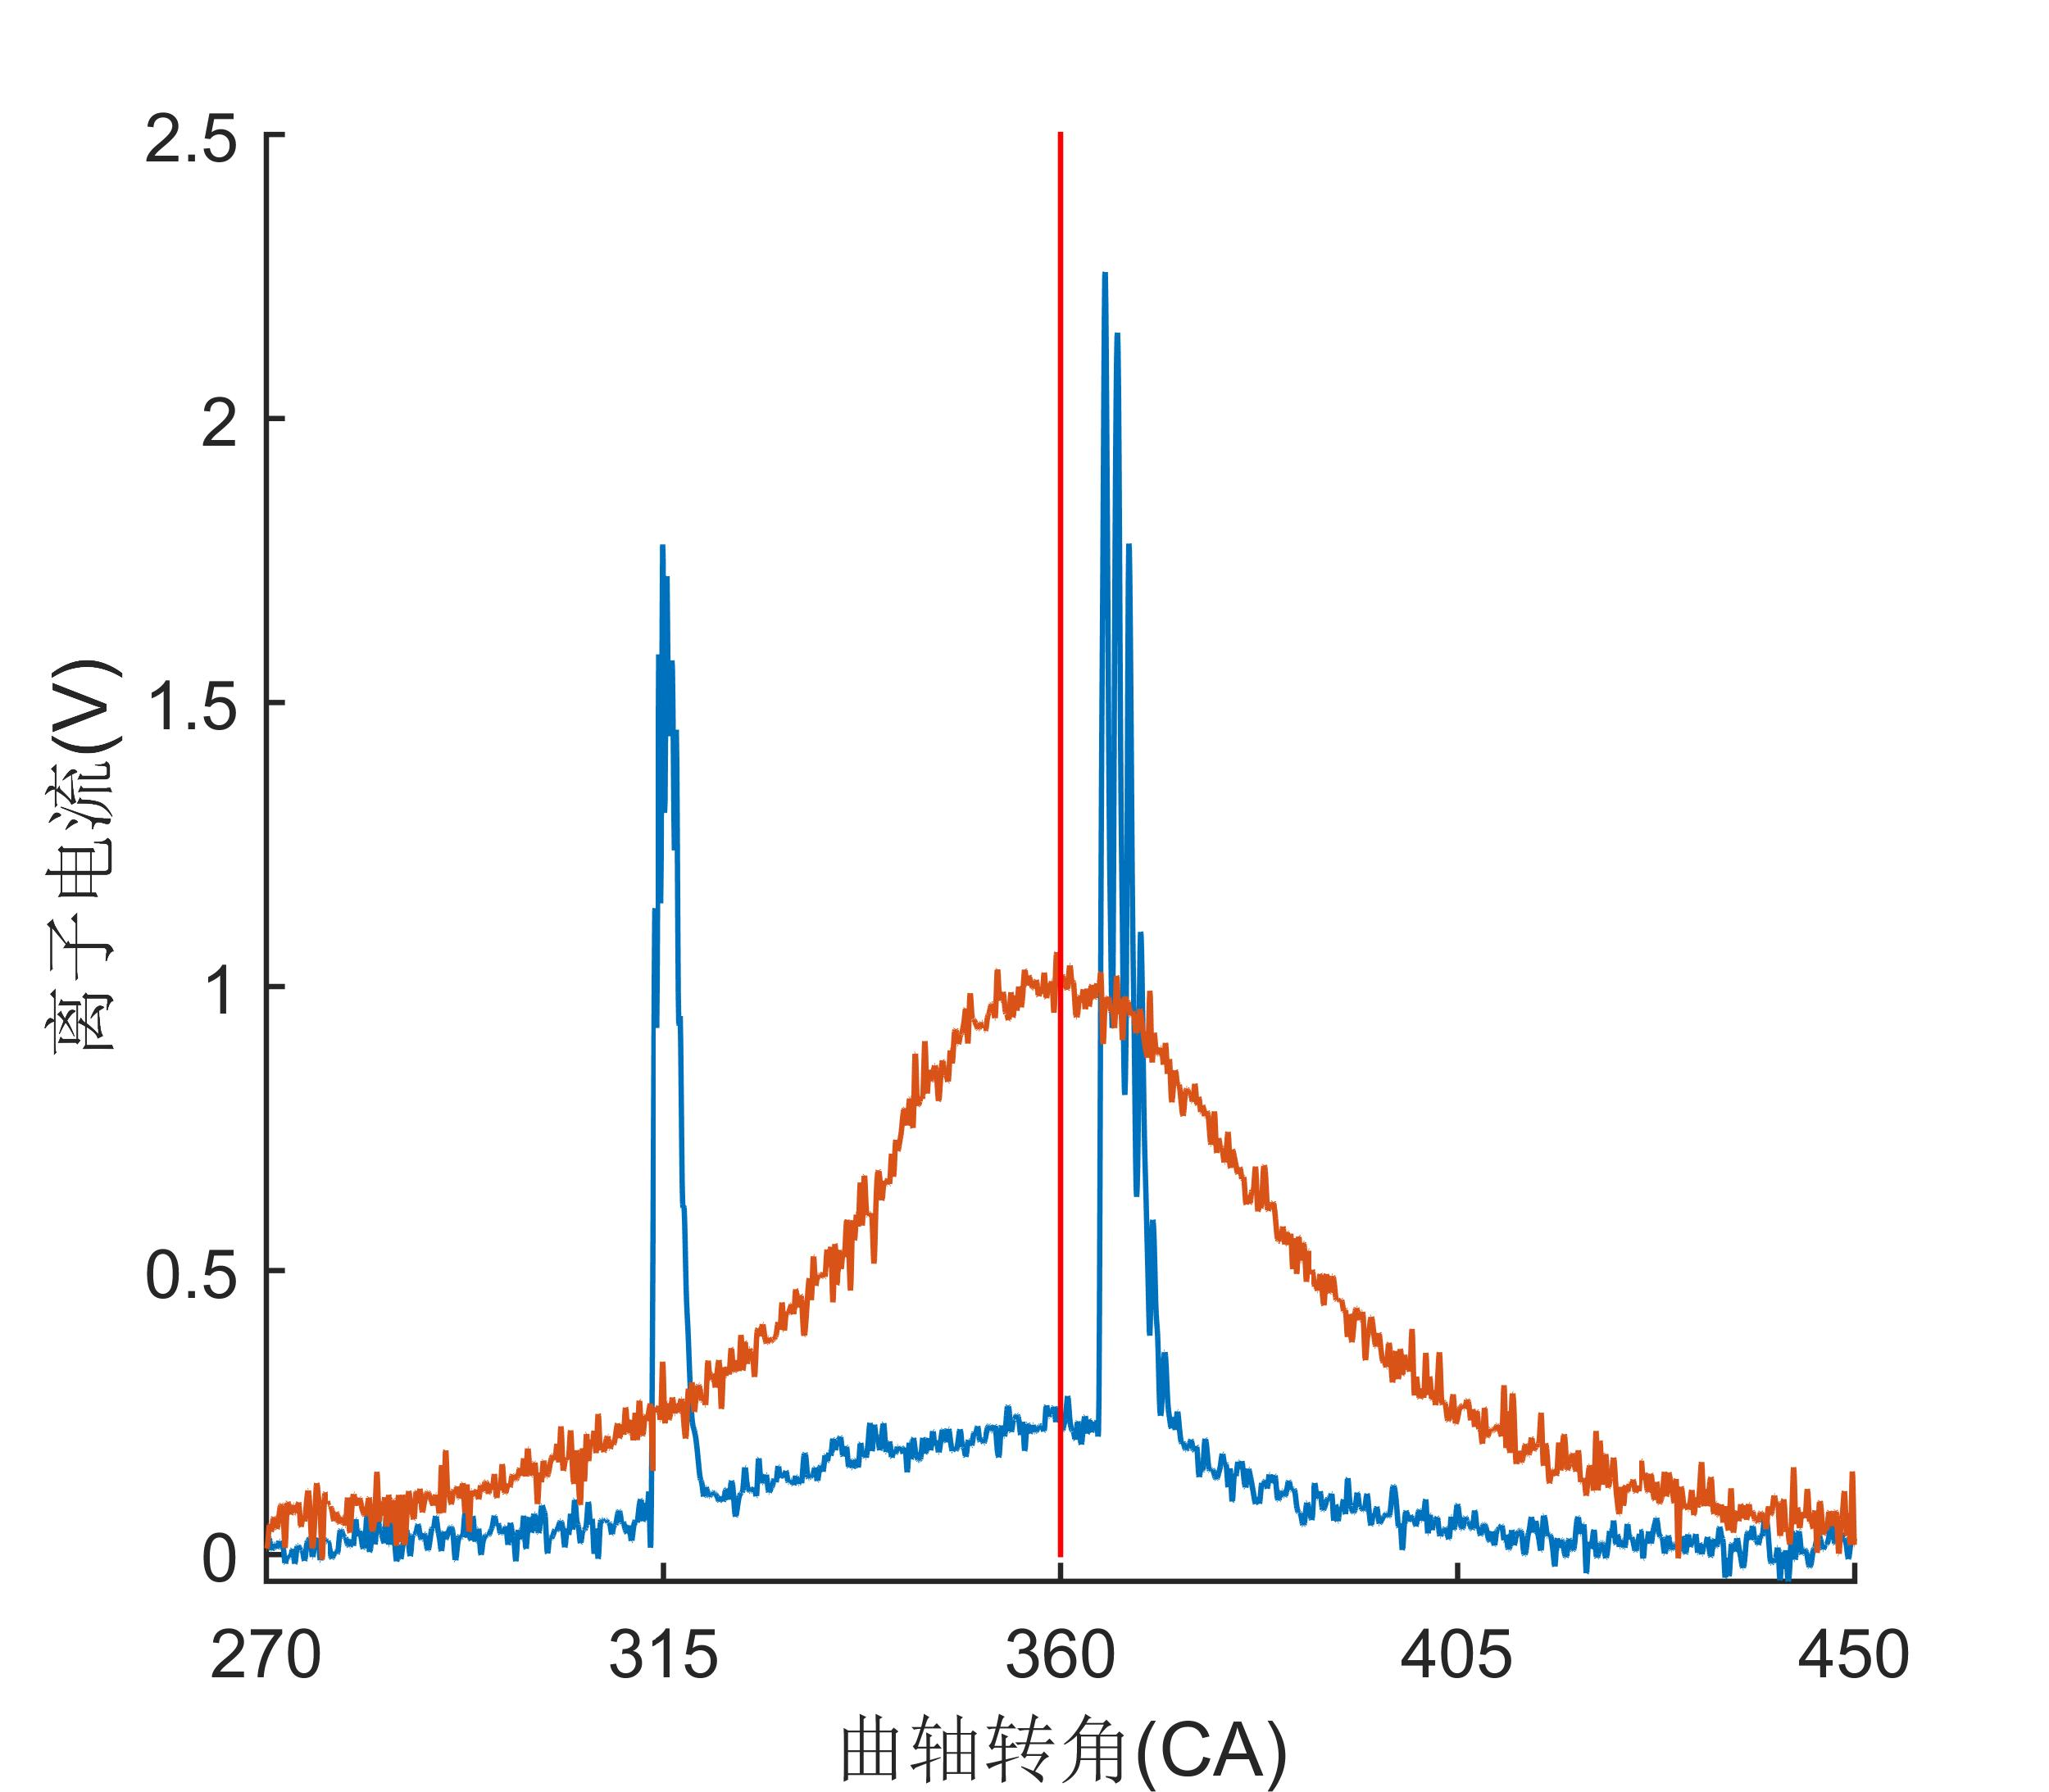
\includegraphics[width=\textwidth]{thesis_figure/ion_chapter/dy_ion}
	\caption{断油情况下的电压信号}
	\label{fig:dy_ion}
\end{minipage}
\begin{minipage}[t]{0.5\linewidth}
	\centering
	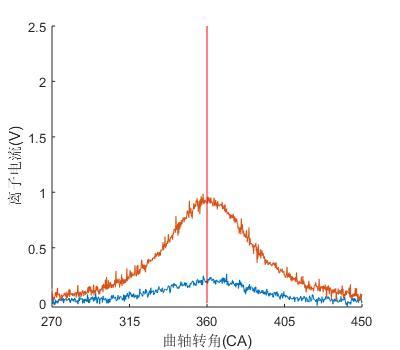
\includegraphics[width=\textwidth]{thesis_figure/ion_chapter/dh_ion}
	\caption{断火情况下的电压信号}
	\label{fig:dh_ion}
\end{minipage}
\end{figure}
\subsection{断火情况下的离子电流分析}   
当发动机断火情况下,点火线圈不进行点火过程,导致缸内混合气不能进行燃烧过程,无法形成化学电离过程的离子电流信号如图\ref{fig:dh_ion}所示是一个断火情况下的电容式检测电路检测到的电压信号。
\par 从图\ref{fig:dh_ion}中可以看到缸压曲线峰值相位在上止点360度位置,说明该循环处于纯压缩循环。可以看到此时的离子电流信号的峰值相位也是上止点位置,此时的离子电流信号是热电离导致的,没有化学电离产生的离子电流信号。
\begin{figure}[htb]
\begin{minipage}[t]{0.5\linewidth}
	\centering
	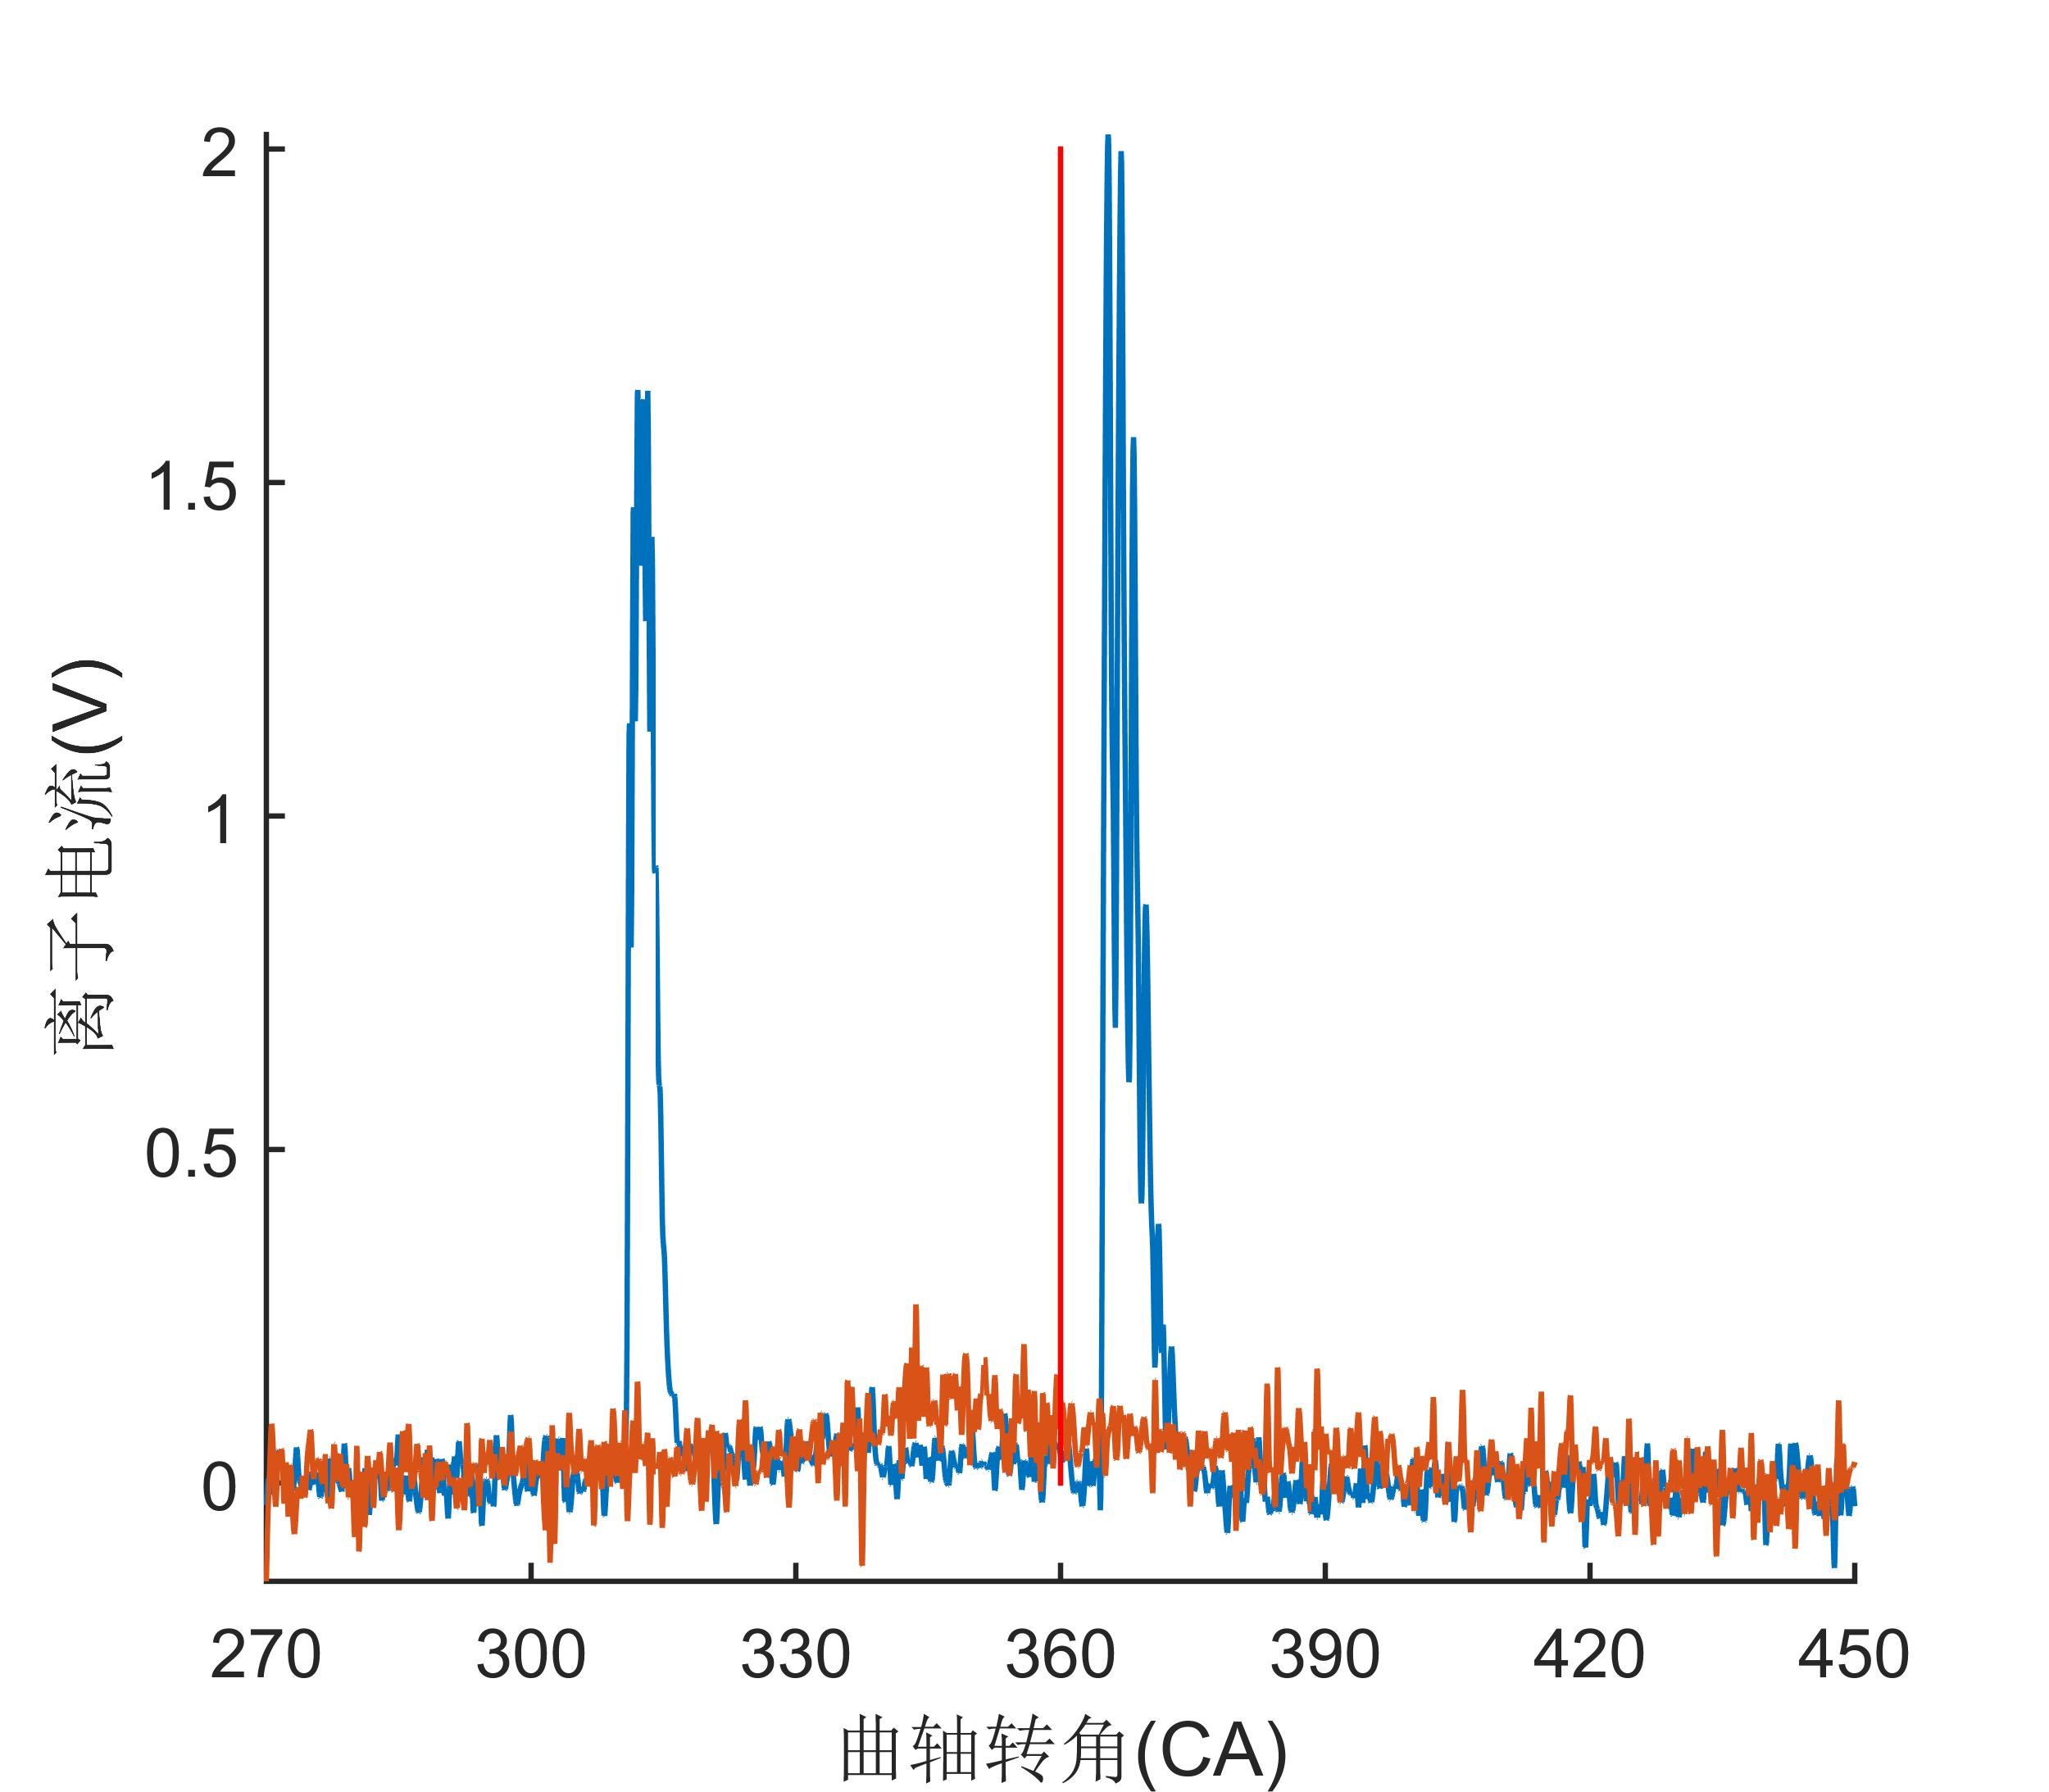
\includegraphics[width=\textwidth]{thesis_figure/ion_chapter/diff_dy_dh}
\end{minipage}
\begin{minipage}[t]{0.5\linewidth}
	\centering
	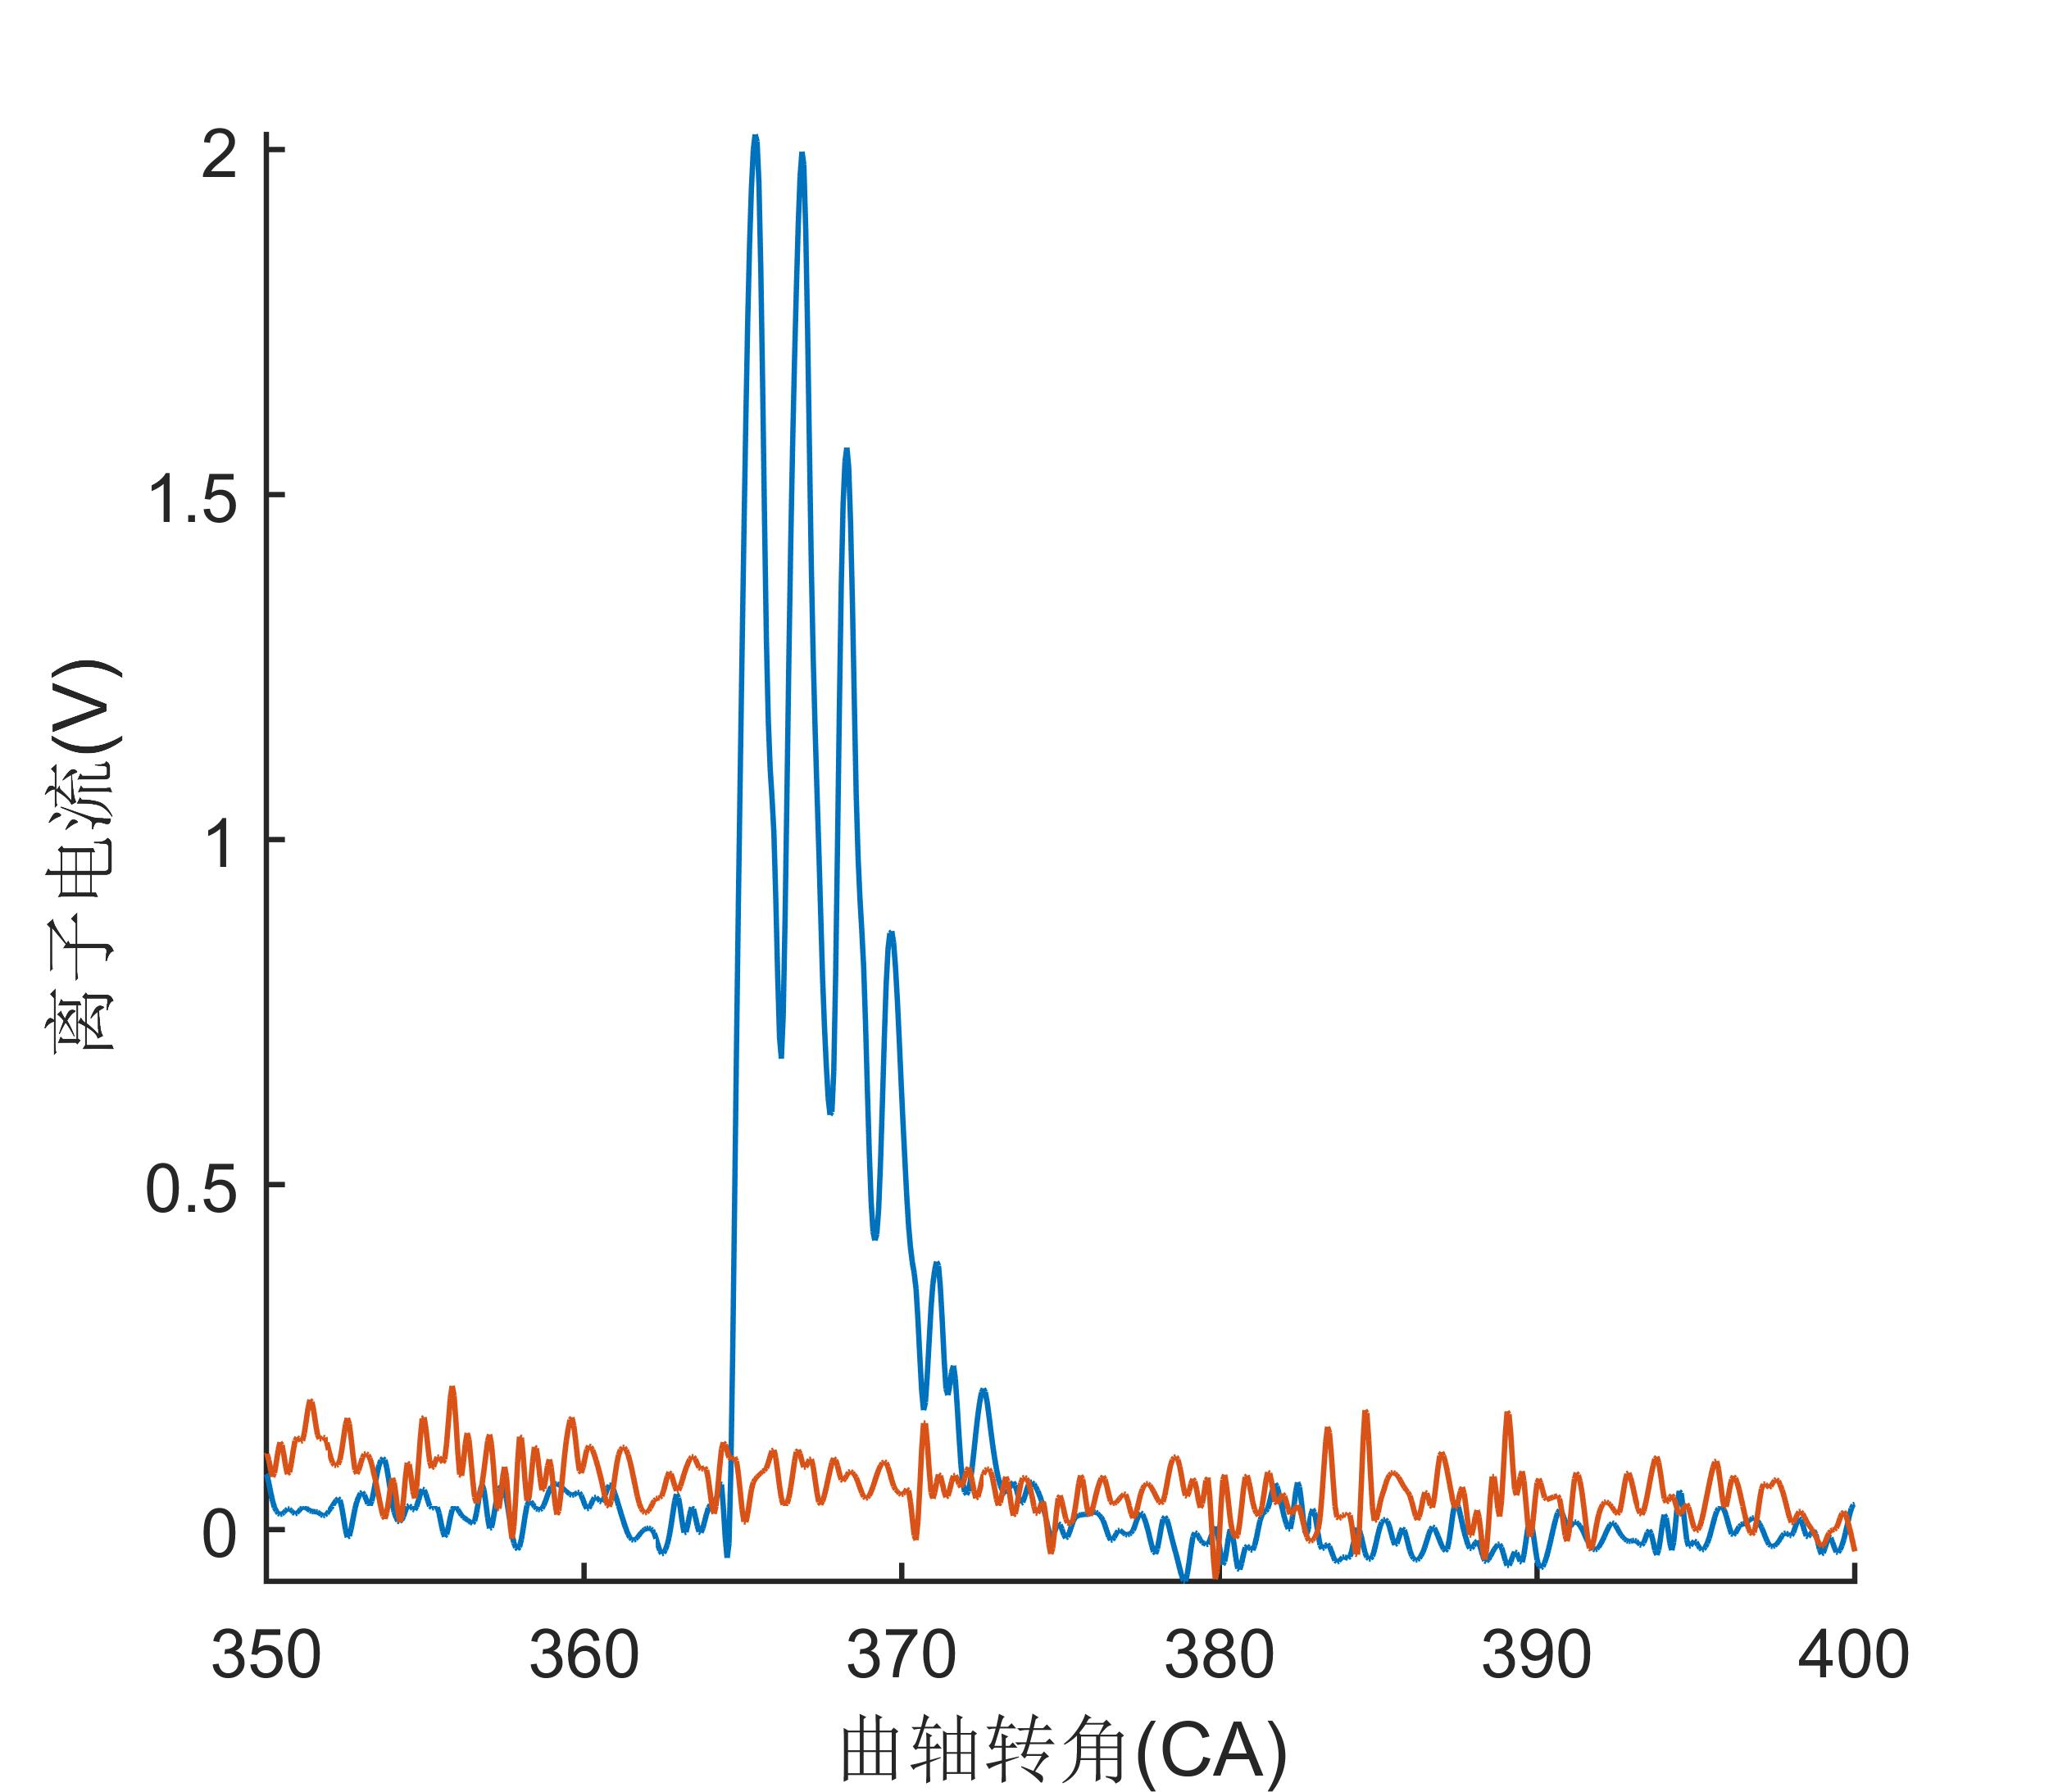
\includegraphics[width=\textwidth]{thesis_figure/ion_chapter/diff_dy_dh_detail}
\end{minipage}
	\caption{断油离子电流信号与断火离子电流信号差值}
	\label{fig:diff_dy_dh}
\end{figure}
\subsection{纯点火干扰的分析}
对比图\ref{fig:dy_ion}和图\ref{fig:dh_ion},可以看到无论断油还是断火,都会导致缸内的混合气体无法燃烧,不能够产生化学电离,两者的循环都是纯压缩循环。
同时非NO热电离曲线的形状和峰值大小都类似。所以可以将同一转速和负荷下的离子电流信号相减,即可得到近似的纯点火干扰信号。
如图\ref{fig:diff_dy_dh}所示可以得到近似的纯点火干扰信号。可以看到两者的缸压曲线的差值几乎为零,说明在同一个工况下的断油和断火循环,造成的缸内情况是类似的,因此两者相减得到的离子电流信号在一定
程度上是可以表征纯电火干扰信号的。
\section{离子电流的小波分析方法}
\subsection{纯点火干扰信号的小波分析} 
小波分析的方法可以很好的将高频信号和低频信号进行分离,采用db,sym,coif,dmey四种离散小波基函数对纯点火干扰信号进行分析,将纯点火干扰信号中的震荡信号去除。
先用dmey小波对纯点火干扰信号进行10层分解,观察第二层到第七层的分解情况,可以得到如图\ref{fig:pure_ign_analysis_dmey}所示的曲线,可以看到第二层和第三层并没有将震荡信号分解开来,
而第六层和第七层分解出来的平滑信号过
于硬直,且分解的震荡信号不具有很好的衰减特性。而第四层分解相对于第五层分解来说,效果没有那么理想。\par
所以本文以下的小波分析都是基于第五层分解来进行的。由于dmey没有阶数问题,而coif小波
的最高阶数为5。因此需要确定db小波和sym小波的阶数,从而可以比较四种小波基函数对离子电流信号分析效果。
\subsection{db小波族的阶数选择和分析} 
取阶数分别为5、10、15、20、25和30的db小波对纯干扰信号进行分析。
从图\ref{fig:dbvar}中可以看到当阶数增加后,小波第五层分解的结果不变,考虑到分解阶数越多计算越加复杂。因此
db小波的阶数可以取20左右的整数值。
\subsection{sym小波族的阶数选择和分析} 
取阶数分别为5、10、15、20、25和30的sym小波对纯干扰信号进行分析。
从图\ref{fig:symvar}中可以看到当阶数增加到20以后,小波分析第五层分解的结果已经基本不变了,而且随着阶数的增加,sym小波分解的时间增加很快。因此
sym小波的阶数可以取20左右的整数值。
\begin{figure}[H]
	\includegraphics[width=\textwidth]{thesis_figure/ion_chapter/pure_ign_analysis_dmey}
	\caption{\label{fig:pure_ign_analysis_dmey}dmey小波对纯点火干扰信号小波分解}
\end{figure}
\begin{figure}[H]
	\centering
	\includegraphics[width=\textwidth]{thesis_figure/ion_chapter/pure_ign_analysis_db_order}
	\caption{\label{fig:dbvar}不同阶数下的db小波第五层分解}
\end{figure}
\begin{figure}[H]
	\centering
	\includegraphics[width=\textwidth]{thesis_figure/ion_chapter/pure_ign_analysis_sym_order}
	\caption{\label{fig:symvar}不同阶数下的sym小波第五层分解}
\end{figure}
\subsection{小波去除纯点火干扰的算法}
根据前三节可以知道,采用db15,sym15,coif5和dmey小波基函数对离子电流信号进行第5层分解可以很好的将震荡信号分离出来。
去除纯点火干扰的方法为用同一个小波基函数对离子电流信号和纯点火干扰信号进行分析,可以将两者的震荡信号分别提取出来得到剩余的曲线,然后两者做差值得出理想的离子电流信号。\par
\begin{figure}[H]
	\centering
	\includegraphics[width=\textwidth]{thesis_figure/ion_chapter/dmey_demo}
	\caption{\label{fig:dmey_realIon}dmey小波分解的真实离子电流信号}
\end{figure}
如图\ref{fig:dmey_realIon}所示的用dmey小波基函数
进行五层小波分析得到的干扰第一峰对比、干扰第二峰对比、提取震荡对比、提取真实离子电流对比以及原信号和提取信号比较图。\par
此时的工况为$1000r/min$、40\%负荷,如左侧第三图所示在此工况下热电离产生的波峰不会被点火干扰淹没。从右侧第三图中可以看到提取信号可以很好的和原离子电流的其他信号部分进行衔接。\par
左侧第一图显示的是干扰第一峰的对比图,可以看到纯点火干扰信号和离子电流信号的干扰第一峰相近,两者的差值几乎为零。右侧第一图显示的是干扰第二峰的对比图,可以看到两者的差值仍然存在
很强的震荡信号,和真实信号有偏差。\par
左侧第二图显示的是提取震荡的对比,可以看到从纯点火干扰中提取到的震荡信号和离子电流信号中提取到的震荡信号在频率和振幅上几乎一样,两者的差值几乎为零。
这说明了用小波分析的方法对点火干扰进行去除有很好的效果,可以提取出真实的离子电流信号出来。
\subsection{四种小波对去除点火干扰分析的比较}
如图\ref{fig:diff_wv_comp}所示是四种小波对真实离子电流进行处理后的信号比较。
\begin{figure}[H]
	\centering
	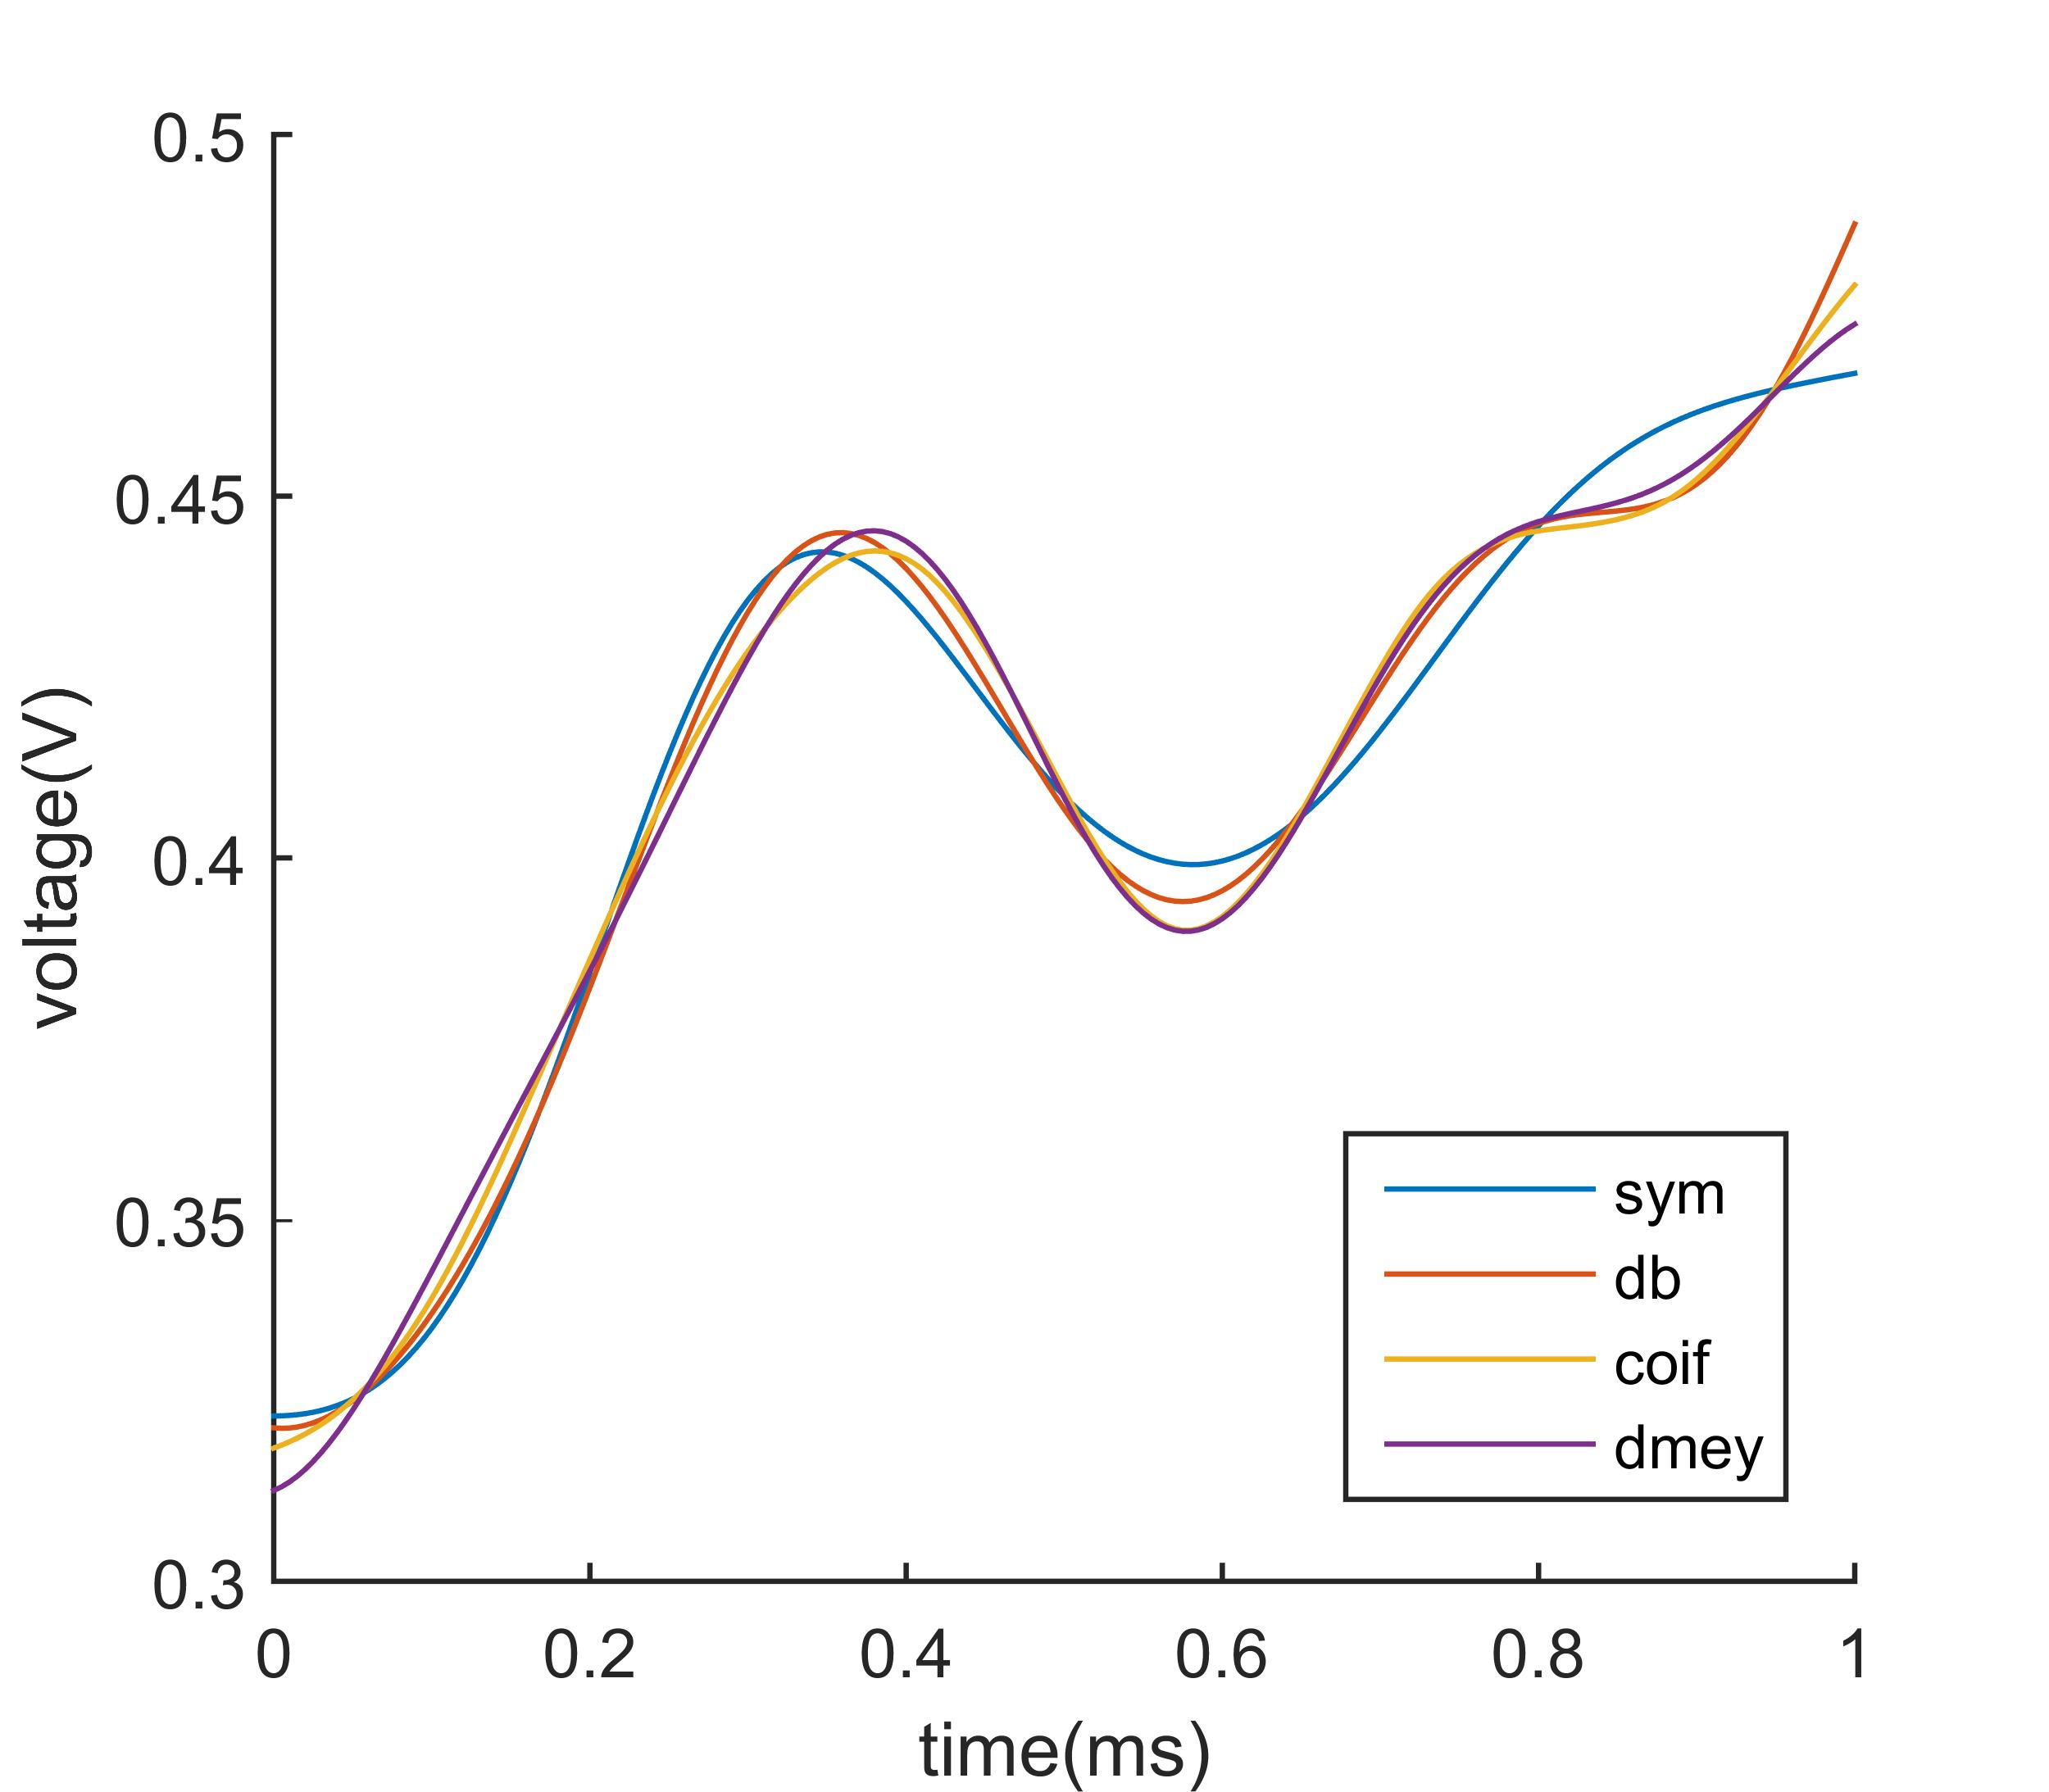
\includegraphics[width=0.8\textwidth]{thesis_figure/ion_chapter/diff_wv_comp}
	\caption{\label{fig:diff_wv_comp}四种小波对真实离子电流进行去干扰处理}
\end{figure}
从图\ref{fig:diff_wv_comp}中可以看到四种小波基函数都能够很好的将离子电流的震荡信号分离提取出平滑的曲线。但是如表\ref{wv_diff}所示的运行时间来看,
从时间对比可以看出采用dmey小波函数进行小波分析的速度最快。因此在本文之后的小波基函数的选择上都采用dmey小波基函数的第五层近似分解作为小波分析的提取结果。
\begin{table}[!htb]
	\centering
	\caption{\label{wv_diff}四种小波基函数计算时间}
	\begin{tabular}{ccc}
		\toprule[1.5pt]
		小波名称&时间(s)&\\
		\midrule[1pt]
		dmey & 0.002&    	\\
		coif & 0.008&     	\\
		db   & 0.019&		\\
		sym  & 0.131&		\\
		\bottomrule[1.5pt]
	\end{tabular}
\end{table}
\section{高斯曲线拟合估计离子电流}
给定在$1750r/min$、40\%负荷时的经过小波分析去除干扰的离子电流,采用附录\ref{cd:dgauss}中的MATLAB代码进行
双高斯曲线的拟合分析得到图\ref{fig:gas_fit_asys}所示的曲线。
\begin{figure}[htb]
	\centering
	\includegraphics[width=0.8\textwidth]{thesis_figure/ion_chapter/gas_fit_asys}
	\caption{\label{fig:gas_fit_asys}双高斯曲线拟合处理}
\end{figure}
由于发动机循环中0到270度为进气和压缩冲程,450度到540度之间基本上没有任何燃烧,540度到720度是排气冲程。所以只有在270度到450度这180度之间才有缸压和离子电流信号,这和实际
测得的信号吻合。因此曲线拟合过程可以只考虑在该相位区间中的信号。\par
从图\ref{fig:gas_fit_asys}中可以看到,火焰后期的峰十分的明显,但是火焰前锋期并不是明显,而只能观测到一段斜率明显的曲线。
纯压缩过程形成的离子电流曲线也能够很好的用高斯函数进行近似拟合,且其形成的原理和热电离的原理是相同的。
\section{本章总结}
本章提出了电容式离子电流检测电路的局限性所在,当转速增加时,点火干扰会将正常的离子电流信号淹没,从而无法准确获得正确的离子电流特征参数。首先从次级电压曲线角度考虑,发现次级电压中的震荡
电压信号是导致离子电流信号中存在点火干扰的直接原因。通过分析断油情况下的离子电流和断火情况下的离子电流,发现两者相减可以得到纯点火干扰信号。由于纯点火干扰信号是由于点火线圈导致的,其具有
稳定的周期和频率,因此具有稳定的特征。通过对纯点火干扰信号的研究,有助于将该信号从离子电流信号中去除。\par
离散小波函数只有db、sym、coif和dmey四种,将这四种小波基函数分别应用于纯点火干扰信号和离子电流信号中,可以将各自的震荡信号提取出来得到各自的近似信号。这两个近似信号相减得到了离子电流的真实
信号,采用该方法就能够将离子电流中的干扰进行去除。同时对比了四种小波基函数在去干扰算法中的优劣,比较结果是采用dmey小波函数有最好的效果。\par
根据离子电流的理论基础可以知道火焰后期的离子电流近似于高斯函数,同时非NO离子的热电离过程也近似于高斯函数,因此可以将整个离子电流信号用两个高斯函数进行近似拟合,便于利用高斯函数的特性
进行快速计算,节省了发动机控制系统的计算资源。\par
本章主要的结论是获得一个完整的计算模型。整个模型可以分为以下几个部分:\par
1)获取单个循环完整的离子电流信号\par
2)采用附录\ref{cd:dintf}中的算法确定两个点火干扰起始位置以及持续时间\par
3)获取在相同工况下的断油、断火离子电流信号从而得到纯点火干扰信号\par
4)通过小波分析方法去除点火干扰\par
5)采用附录\ref{cd:dgauss}中的双高斯曲线拟合算法对离子电流的特征参数进行计算\par
整个模型计算过程适用于任何工况下的离子电流信号。\par
在整个模型的设计过程中,主要的难点在于点火干扰起始位置的确定和小波基函数的选择,因为小波分析过程主要是去除掉
离子电流信号中的震荡成分,真实的离子电流是不存在震荡成分的。而点火干扰起始位置的设定直接影响了截取下来的信号是否完全包含了所有的震荡信号;不仅如此,点火干扰起始位置
设定过早容易让小波分析过程产生偏差,将无震荡信号部分的信号假定为了存在震荡成分。除此之外,双高斯曲线拟合过程也需要优化算法,离子电流信号的不稳定性容易导致
拟合过程产生偏差。\par
\chapter{离子电流的工况拓展}
在上一章中主要探讨的是离子电流未被淹没情况下的离子电流信号分析手段,主要包括小波分析去除干扰,高斯曲线拟合提取离子电流特征参数。
这些手段同样也可以用于淹没情况下的离子电流信号处理,且由于淹没情况下的离子电流信号无法直接提取特征参数,利用上述方法对离子电流信号
进行处理成为了非常有效的手段。本章就这些方法对离子电流工况拓展的可行性进行验证。
\section{离子电流基本特征参数}
离子电流基本特征参数主要包括,火焰前锋期时间$t_c$,火焰前锋期峰值相位$d_c$,火焰后期时间$t_r$,火焰后期峰值相位$d_r$,离子电流积分值$I_i$和离子电流升高率$\phi$等。\par
火焰前锋期与火焰经过电极两段时的火焰前锋面有关,由于时间比较短,而且没有深刻的理论基础,无法很好的得到火焰前锋期的具体形状,从而很难判断火焰前锋期的时间和
峰值相位。西安交通大学的吴筱敏\cite{iign}分析了不同电极间距下的离子电流信号曲线,如图\label{fig:intersection_ign}所示的是改变电极间距$\delta$测量得到的离子电流曲线。
\begin{figure}[!htpb]
	\centering
	\includegraphics[width=0.65\textwidth]{thesis_figure/ion_chapter/intersection_ign}
	\caption{\label{fig:intersection_ign}不同电极间距的离子电流信号曲线}
\end{figure}
从图\label{fig:intersection_ign}中可以看到火焰前锋期只有一个很小的波峰,且随着电极间距离的增加火焰前锋期越加的不明显。若要通过算法计算火焰前锋期很难实现。\par
火焰后期与整个缸内混合气的燃烧过程有关,且根据Andre Saitzkoff\cite{saitzkoff1996ionization}的理论可以知道,火焰后期主要和NO的热电离有关系,其形状近似高斯函数。
因此可以推断火焰后期和滞燃期$t_{\theta_1}$、急燃期$t_{\theta_2}$和后燃期$t_{\theta_3}$有相关性,通常我们采用放热率CA的百分比来定义这几个燃烧的时期,如下公式所示:
\begin{align}
	t_{\theta_1}^{'} &= CA0  & t_{\theta_1}^{''} &=CA10 \\
	t_{\theta_2}^{'} &= CA10 & t_{\theta_2}^{''} &=CA90 \\
	t_{\theta_3}^{'} &= CA90 & t_{\theta_3}^{''} &=CA100 
\end{align}
而根据双高斯曲线拟合方法,可以定义高斯曲线的宽度的两倍即为火焰后期宽度。从而可以根据高斯
曲线的中心位置和宽度计算出火焰后期的开始时刻$t_{r}^{'}$和结束时刻$t_{r}^{''}$。由此可以分析火焰后期和滞燃期$t_{\theta_1}$、急燃期$t_{\theta_2}$、后
燃期$t_{\theta_3}$三者之间的关系。\par
离子电流的积分值$I_i$的计算方式采用去除纯压缩导致的热电离的离子电流积分方式,NO热电离是导致离子电流的主要原因,因此产生NO过程的燃烧对应的做工和离子电流积分值会有对应的关系。\par
离子电流升功率$\phi$的计算方法采用的是用拟合高斯曲线的高度和拟合高斯曲线的宽度的比值。\par
根据以上的总结可以得到离子电流基本特性参数的计算公式如下:
\begin{align}
	t_{r}^{'} &= g_{c}-g_{w}\\
	t_{r}^{''} &= g_{c}-g_{w}\\
	d_{r} &= g_{c}\\
	\phi &= \frac{g_{h}}{g_{w}}\\
	I_{i} &= g_{h}e^{-(\frac{g_c}{g_w})^2}+g_{h}^{'}e^{-(\frac{{g_c}^{'}}{{g_w}^{'}})^2};
\end{align}
其中$g_{c}$,$g_w$,$g_h$分别是火焰后期即第二拟合高斯函数的中心曲轴转角,宽度和高度。$g_{c}^{'}$,$g_w^{'}$,$g_h^{'}$是第一高斯函数的中心曲轴转角,宽度和高度。
其中积分值$I$的计算方法采用的是拟合高斯函数和标准高斯函数的比值来计算,因为标准高斯函数的积分值为1,这样可以大大缩减计算时间。
\section{离子电流工况拓展方法的验证}
采用上一章节中的小波分析方法和双高斯曲线拟合方法来分析离子电流淹没工况下($3000r/min$)的单个随机循环的离子电流,得到如图\ref{fig:5_1_merged_ion}所示的结果。
\begin{figure}[!htb]
	\centering
	\includegraphics[width=\textwidth]{thesis_figure/ion_chapter/5_1_merged_ion}
	\caption{\label{fig:5_1_merged_ion}淹没工况下离子电流的小波分析处理}
\end{figure}
从图\ref{fig:5_1_merged_ion}中可以看到火焰后期的尖峰被分离了出来。从单个循环的角度来看,该离子电流工况拓展方法是有效的,还需要经过多循环分析的讨论。多循环分析主要从两个基本原理和已经
被证实的离子电流特性共三个角度来考虑。\par
第一,从原理的角度上来看,对离子电流信号进行小波分解,将震荡信号消除不会将真实的离子电流信号去除。因为离子电流产生的基本原理是离子的移动,不具有高频往复的特性,不会产生震荡信号。震荡信号的主要
来源是点火线圈的震荡。因此小波分析去除干扰的方法有很强的科学性。\par
第二,从原理的角度上来看,火焰后期主要和NO的热电离有关系,其形状近似高斯函数。火焰后期和滞燃期$t_{\theta_1}$、急燃期$t_{\theta_2}$和后燃期$t_{\theta_3}$有相关性。CA10表征的是滞燃期的开始时刻,而CA90表征
火焰后期的结束时刻。因此CA10和CA90表示的是整个燃烧的开始和结束。考虑离子电流淹没工况下($3000r/min$)通过计算随机连续20个循环的CA10、CA90和火焰后期开始时刻和结束时刻得到
如图\ref{fig:5_1_ca_m2center_start_end}所示的曲线。\par
\begin{figure}[!htb]
	\centering
	\includegraphics[width=0.8\textwidth]{thesis_figure/ion_chapter/5_1_ca_m2center_start_end}
	\caption{\label{fig:5_1_ca_m2center_start_end}CA10、CA90和火焰后期开始时刻和结束时刻}
\end{figure}
从图中可以看到,CA10和火焰后期开始时刻比较吻合,而CA90和火焰后期结束时刻比较吻合。这符合火焰后期主要是燃烧导致的NO电离导致的。\par
第三,根据文献可以知道,火焰后期峰值相位和缸压峰值相位之间有稳定的线性关系,而火焰前锋期峰值相位应该也和缸压的特定点具有稳定的相位关系。从图\ref{fig:5_1_merged_ion}中我们也可以
看到火焰后期的峰值相位和缸压峰值相位之间确实非常的接近。考虑离子电流淹没工况下($3000r/min$)通过计算随机选取的连续20个循环的缸压峰值相位和火焰后期峰值相位图,
可以得到如图\ref{fig:5_1_pph_m2center}所示的曲线。\par
\begin{figure}[!htb]
	\centering
	\includegraphics[width=0.8\textwidth]{thesis_figure/ion_chapter/5_1_pph_m2center}
	\caption{\label{fig:5_1_pph_m2center}缸压峰值相位和火焰后期峰值相位}
\end{figure}
从图\ref{fig:5_1_pph_m2center}中可以看到两者之间有很强的线性关系,且各个循环两者的差值在5度左右,总体的变化趋势保持一致。\par
总结以上三个方面的推导,理论上NO热电离产生的离子电流没有高频信号,经过小波分析得到的离子电流信号的峰值相位和缸压峰值相位有很好的对应关系,对小波分析得到的离子电流信号进行双高斯曲线拟合
计算得到的火焰后期的初始时刻和CA10对应,火焰后期的结束时刻和CA90对应,由此我们可以判定采用小波分析和双高斯曲线拟合方法可以科学准确地计算得到离子电流的特征参数,该离子电流工况拓展的方法具有
科学性和有效性。
\section{高斯拟合曲线计算特征参数}
双高斯曲线拟合方法很好的将非NO热电离产生的离子电流和燃烧产生的NO热电离的离子电流拟合出来,通过拟合曲线的计算可以很好的快速计算出离子电流的特性,从而对缸内的燃烧情况有粗略的掌控。
\subsection{离子电流火焰前锋期的不确定性}
离子电流火焰前锋期很容易被点火干扰和噪声淹没,所以离子电流火焰前锋期的特征参数在较多工况下都是无法获得的\cite{wxm2001,zxc2008}。即使在点火干扰被去除的情况下,有时候也无法很好的获得火焰前锋期的特征参数,
主要原因是火焰前锋期的持续时间较短。火焰前锋期是由火焰锋面经过电极两段时产生的,其原理注定其持续时间较短。且由于缸内湍流燃烧,火焰锋面具有不确定性,同时
火焰锋面的传播过程没有很强的理论支持,不能够通过函数拟合方式很好的获得。
\subsection{火焰后期近似计算与急燃期}
通过缸压计算CA10和CA90,通过高斯拟合曲线计算火焰后期高斯拟合峰的初始位置和结束位置,得到如图\ref{fig:ca10_ca90_m2s_m2e}所示。可以看到CA10和火焰后期的初始
时刻对应,CA90和火焰后期的结束时刻对应。
\begin{figure}[!htb]
	\centering
	\includegraphics[width=0.8\textwidth]{thesis_figure/ion_chapter/ca10_ca90_m2s_m2e}
	\caption{\label{fig:ca10_ca90_m2s_m2e}CA10、CA90和火焰后期开始时刻和结束时刻}
\end{figure}
\subsection{峰值相位的近似计算}
通过计算随机选取的$3000r/min$淹没工况下的连续20个循环的离子电流火焰后期峰值相位和缸压峰值相位可以得到如图\ref{fig:ionpph_pph}所示的曲线。可以看到离子电流火焰后期
峰值相位和缸压峰值相位有一定的相关性。
\begin{figure}[htb]
	\centering
	\includegraphics[width=0.8\textwidth]{thesis_figure/ion_chapter/ionpph_pph}
	\caption{\label{fig:ionpph_pph}离子电流火焰后期峰值相位和缸压峰值相位}
\end{figure}
\subsection{积分值的近似计算}
纯点火干扰的存在影响了离子电流积分值的计算,且由于点火干扰的不稳定性,其积分值也是不稳定的。若将干扰的积分值计算在内,并不能很好的表征离子电流的真实积分值。
采用小波分析方法将点火干扰去除,再经过积分计算得到的离子电流积分值有很强的科学性。\par
通过计算随机选取的$3000r/min$淹没工况下的连续20个循环的离子电流积分值和IMEP可以得到如图\ref{fig:integer_imep}所示的曲线。可以发现离子电流和IMEP有一定的相关性。\par
\begin{figure}[htb]
	\centering
	\includegraphics[width=0.8\textwidth]{thesis_figure/ion_chapter/gausint_imep}
	\caption{\label{fig:integer_imep}离子电流积分值和IMEP}
\end{figure}
通过分别计算随机选取的$3000r/min$淹没工况下的连续20个循环的小波分析后的离子电
流积分值和双高斯曲线的积分值,可以得到如图\ref{fig:ionint_gaussint}所示的曲线。
\begin{figure}[htb]
	\centering
	\includegraphics[width=0.8\textwidth]{thesis_figure/ion_chapter/ionint_gaussint}
	\caption{\label{fig:ionint_gaussint}离子电流积分值和高斯拟合积分值}
\end{figure}
可以发现两者之间几乎相等,说明用双高斯曲线计算的积分值可以非常好的表示离子电流积分值。
因此可以用双高斯曲线计算的积分值来近似得到对应的IMEP值,而高斯曲线的面积计算有快速算法,由此在没有安装缸压传感器的发动机上可以非常快速的计算得到IMEP的值。
\begin{figure}[htb]
	\centering
	\includegraphics[width=0.8\textwidth]{thesis_figure/ion_chapter/prr_irr}
	\caption{\label{fig:prr_irr}离子电流升高率和缸压升高率}
\end{figure}
\subsection{升高率的近似计算}
通过分别计算随机选取的$3000r/min$淹没工况下的连续20个循环的小波分析后的离子电流升高率和缸压升高率,可以得到如图\ref{fig:prr_irr}所示的曲线。可以发现
离子电流升高率和缸压升高率有一定的相关性。\par
通过分别计算随机选取的$3000r/min$淹没工况下的连续20个循环的小波分析后的离子电流最大升高率相位和最大缸压升高率相位,可以得到如图\ref{fig:prrph_irrph}所示的曲线。
可以发现离子电流最大升高率相位和最大缸压升高率相位有一定的相关性。
\begin{figure}[htb]
	\centering
	\includegraphics[width=0.8\textwidth]{thesis_figure/ion_chapter/prrph_irrph}
	\caption{\label{fig:prrph_irrph}最大离子电流升高率相位和最大缸压升高率相位}
\end{figure}
\section{估计特征参数的相关性和循环变动}
循环变动系数\cite{xhbd}采用发动机中常用燃烧循环变动算法,循环变动系数的定义如下:
\begin{align}
	CoV_x = \frac{\sigma_x}{\overline{x}}
\end{align}
式中$x$是任一物理量,$\sigma_x$是该物理量的标准偏差,$\overline{x}$是该物理量的平均值,其计算公式为
\begin{align}
	\sigma_x &= \sqrt{\sum_{i=1}^{N}(x-\overline{x})^2}\\
	\overline{x} &= \frac{\sum_{i=1}^{N}x_i}{N}
\end{align}
选取随机20个循环计算双高斯曲线估计特征参数与真实信号特征参数的相关性,并计算循环变动率可以得到如表\ref{tab:parainfo}所示的表格。
而经过计算的缸压循环变动率为4.7\%,可以发现除了离子电流的积分值估计值和升高率估计值,其他的循环变动
都比缸压的循环变动率低,因此可以说明双高斯曲线拟合计算得到的特征值估计具有很好的稳定性\cite{ljw2005}。\par
从相关性角度来看,火焰后期峰值相位、离子电流积分值和离子电流升高率相位具有明显的相关性;火焰后期初始时刻、火焰后期结束时刻
和离子电流升高率有一定地相关性\cite{joyce2006linear}。
\begin{table}[H]
	\centering
	\caption{\label{tab:parainfo}特征参数估计值的相关性和循环变动系数}
	\begin{tabular}{ccc}
		\toprule[1.5pt]
		特征参数估计值&相关性&循环变动系数(\%)\\
		\midrule[1pt]
		火焰后期初始时刻&0.12&1.8\\
		火焰后期结束时刻&0.18&1.7\\
		火焰后期峰值相位&0.47&0.4\\
		积分值&0.44&5.12\\
		升高率&0.21&5.6\\
		升高率相位&0.68&0.9\\
		\bottomrule[1.5pt]
	\end{tabular}
\end{table}
\section{本章总结}
本章总结并分析了离子电流的基本特征参数,以及通过拟合曲线对特征参数的计算方法。\par
由于原理上看,离子电流信号不具有高频信号成分;离子电流的产生是由于燃烧产生的NO离子电离导致的,因此离子电流
的开始时刻、结束时刻和燃烧的开始时刻、结束时刻是一一对应的;且离子电流火焰后期峰值相位和缸压峰值相位有线性相关性。本章从这三个角度应证了小波分析和双高斯曲线拟合方法可以很好的对离子电流
进行拟合。\par
本章最后通过拟合曲线计算了离子电流曲线的不同特征参数,多循环角度分析了离子电流的特性和缸压特性,得出了许多有用的离子电流特性,为离子电流更深层次的应用打下了理论基础。
本章得到的主要结论如下:\par
(1)离子电流火焰后期峰值相位和缸压峰值相位有明显的相关性。\par
(2)离子电流火焰后期的开始时刻、结束时刻和缸内燃烧的开始时刻、结束时刻有一定的相关性。\par
(3)双高斯拟合曲线的积分值与离子电流积分值基本相等,且和IMEP有很好的明显的相关性。\par
(4)缸压最大压力升高率和离子电流火焰后期最大升高率有一定的相关性。缸压最大压力升高率相位和离子电流火焰后期最大升高率相位有明显的相关性。\par
(5)离子电流积分值和升高率估计值有一定波动,其他特征值的估计值都具有很好的稳定性。
\chapter{总结及展望}
\section{全文总结}
目前,国内外对离子电流基本特性的研究很多,电容式离子电流检测电路具有性价比高,安装方便的特点,但是由于没有屏蔽点火干扰,随着转速的增加,容易造成点火干扰淹没正常的离子电流信号的弊端。
本文通过小波分析的方法很好的将离子电流信号中的点火干扰信号分离出去,获得了理想的离子电流信号。同时比较不同的小波基函数以及小波分析层级,得出了最佳的小波基函数和分解层数。
同时采用了双高斯拟合算法,能够快速地计算出离子电流的各种特征值,能够大大缩小需要的发动机控制系统的计算资源;比较了特征值的估计值和真实值之间的相关性和循环波动率,验证了
双高斯曲线拟合算法估算离子电流特征值的有效性。\par
本文通过小波分析方法和双高斯曲线拟合方法对离子电流的火焰后期峰值、火焰后期时间、离子电流积分值和离子电流升高率等进行了分析,得到了如下的结论:\par
(1)点火干扰信号是由点火线圈产生的,具有稳定的频率特性和振幅特性。离子电流是由于燃烧产生的离子在电场的作用下的移动产生的,不具有震荡信号成分。因此从采集到的离子电流信号中分离出
具有震荡特性的点火干扰信号具有坚定的理论基础。\par
(2)小波分析方法通过小波基函数逐层对信号进行对比分离出近似信号和细节信号,能够很好地提取出信号中的震荡成分。采集信号是离散信号,需要使用离散小波基。比较四种常用的离散小波基和十层小波分解发现
采用dmey小波基函数和第五层近似分解可以很好地去除点火干扰信号,提取出真实的离子电流信号。\par
(3)根据离子电流的理论原理,火焰后期由NO离子的热电离导致的信号近似高斯函数,可以用高斯曲线近似分析。而由于排气过程不能将缸内的所有废弃排除缸内,断油循环和断火循环中仍然存在部分带NO离子
的废弃,仍然可以检测到离子电流。同样道理,在正常循环的点火之前由于存在部分废气,离子电流检测电路可以检测到轻微的离子电流信号。这部分废弃导致的离子电流信号也可以用高斯函数近似分析。
由此整个检测到的离子电流信号可以用两个高斯曲线拟合来进行分析。\par
(4)利用双高斯曲线拟合得到的离子电流特征参数估计值和缸压特征值有相关性。离子电流的火焰后期峰值相位估计值和缸压峰值相位明显的相关性;离子电流的火焰后期开始时刻估
计值、结束时刻估计值和燃烧放热率CA10、CA90有一定的相关性;离子电流积分值估计值和平均指示压力有明显的相关性;最大离子电流升高率估计值和最大缸压升高率有一定的相关性;
最大离子电流升高率对应曲轴转角估计值和最大缸压升高率对应曲轴转角有明显的相关性。\par
(5)离子电流积分值和升高率估计值有一定波动,其他特征值的估计值都具有很好的稳定性。
\section{工作展望}
本文的实验和拟合计算方面还有很多地方可以提高,主要有:\par
(1)电磁屏蔽\cite{cyb2012,tb2009}做得不够细致导致采集信号的噪声信号过大,导致通过差值计算得到的纯点火干扰信号夹杂噪声,会在一定程度上影响小波分析提取真实离子电流信号的效果;\par
(2)废气产生的热电离信号可以用其他函数来进行近似计算;\par
(3)两个点火干扰信号起始位置计算的算法需要优化,对真实信号和纯点火干扰信号做小波分析后相减的算法对点火干扰信号的起始位置计算要求很高;

%%% 其它部分
\backmatter
\makeatother

% 致谢
% !TeX encoding = GB2312

%%% Local Variables:
%%% mode: latex
%%% TeX-master: "../main"
%%% End:

\begin{ack}
  ���ĸ�л��ʦ��־�����ڶԱ��˵ľ���ָ�������ǵ��Դ����̽�ʹ
  ���������档

  ��������ʡ����ѧԺ��ѧϵ���оŸ��µĺ����о��ڼ䣬���� xxx ��������ָ�����������
  ʤ�м�����л xx ʵ�������� xx ���ڣ��Լ�ʵ����ȫ����ʦ��ͬѧ�ǵ����������֧
  �֣���������ɹ�����Ȼ��ѧ�����������ش���л��

  ��л \tongjithesis{}�����Ĵ������ҵ�����д���������������࣬���ҵ����ĸ�ʽ����Ư����
  ���ࡣ

\end{ack}


% 参考文献
\bibliographystyle{tongjibib}
\bibliography{ref/ref_thesis}

% 附录
%\begin{appendix}
%\chapter{部分代码文件}
\section{离子电流双干扰确定算法}
\label{cd:dintf}
\lstset{
	basicstyle=\ttfamily\scriptsize,
	breaklines=true}
	
\begin{lstlisting}[frame=single,language=matlab]
function [fA,fB]=fluccalc(y,dA,dB)
% y	data of ion of a single cycle
% dA 	the offset of interfere A
% db 	the offset of interfere B
% fA 	struct for start point and stop point of interfere A
% fB 	struct for start point and stop point of interfere B
switch nargin
    case 1
        dA = 0; dB = 0;
    case 2
        dB = 0;
    otherwise
end

y_a = dgtflt(diff(y));

for num = 1:length(y_a)
    if y_a(num)>0.1
        flucAStart = num+dA;
        break;
    end
end

for num = (flucAStart+200):-1:flucAStart
    if y_a(num)>0.1
        flucAEnd = num;
        break;
    end
end

for num = (flucAStart+200):length(y)
    if y_a(num) >0.1
        flucBStart = num+dB;
        break;
    end
end

flucBEnd = flucBStart+200;

fA = struct('fAs',flucAStart,'fAe',flucAEnd);
fB = struct('fBs',flucBStart,'fBe',flucBEnd);
\end{lstlisting}
\section{双高斯曲线拟合算法}
\label{cd:dgauss}
\lstset{
	basicstyle=\ttfamily\scriptsize,
	breaklines=true}
	
\begin{lstlisting}[frame=single,language=matlab]
function [lambda,A,peakHeights] = iongaussfit(y)
	% y         ion data sequence from 270 to 450 degree.
	% lambda    a matrix of 2x2, each row is responsive to a gaussian curve
	global numpeaks ns pos1 pos2;
	ns = 1:length(y);
	numpeaks = 2;
	[~,tempos] = max(y);

	%gaussian parameter initial setting
	pos1 = round(length(y)/2); % pos1 = 360 dgr
	pos2 = tempos; % pos2 = the maximum value of ion
	slambda = [pos1,1200,pos2,100];

	options = optimset('TolX',.00001,'Display','iter' );
	lambda = fminsearch(@fitgaussian,slambda,options,y);

	A(:,1) = gaussian(ns,lambda(1),lambda(2));
	A(:,2) = gaussian(ns,lambda(3),lambda(4));

	peakHeights = abs(A\y);

	test(A,peakHeights,y); %plot model and each gaussian curve
end

function err = fitgaussian(lambda,y)
	global ns;
	A(:,1) = gaussian(ns,lambda(1),lambda(2));
	A(:,2) = gaussian(ns,lambda(3),lambda(4));

	peakheights = abs(A\y);
	z = A*peakheights;
	err = norm(z-y);
end

function g = gaussian(x,pos,wid)
	g = exp(-((x-pos)./(0.6005615.*wid)) .^2);
end

function test(A,peakHeights,y)
	% TEST SCRIPTS
	global numpeaks;
	mmodel = A*peakHeights;
	rge = (1:length(y))*180/length(y)+270;
	
	figure('unit','centimeters','position',[2 2 14.6*0.8 8]);hold on;
	plot(rge,mmodel,'r');plot(rge,dgtflt(y,4),'b');
	
	for j=1:numpeaks;
		plot(rge,peakHeights(j)*A(:,j));
	end
	
	legend('sim model','real','gauss1','gauss2');
	xlabel('crank angle(CA)');ylabel('ion voltage(V)');
	ylim([0 1]);xlim([270 450]);
	set(gca,'fontsize',8,'xtick',270:30:450);

end
\end{lstlisting}
%\end{appendix}

% 个人简历
% !TeX encoding = GB2312
\begin{resume}

  \resumeitem{���˼���}

  xxxx �� xx �� xx �ճ����� xx ʡ xx �ء�
  
  xxxx �� 9 �¿��� xx ��ѧ xx ϵ xx רҵ��xxxx �� 7 �±��Ʊ�ҵ����� xx ѧʿѧλ��
  
  xxxx �� 9 �����Խ��� xx ��ѧ xx ϵ���� xx ѧλ����

  \resumeitem{������ѧ������} % �����ĺ�¼�õĺ���һ��

  \begin{enumerate}[{[}1{]}]
  \item Yang Y, Ren T L, Zhang L T, et al. Miniature microphone with silicon-
    based ferroelectric thin films. Integrated Ferroelectrics, 2003,
    52:229-235. (SCI ��¼, ������:758FZ.)
  \item ����, ������, ������, ��. �������΢��ѧ�����б�Ĥ����Ӧ�����о�. �й���
    е����, 2005, 16(14):1289-1291. (EI ��¼, ������:0534931 2907.)
  \item ����, ������, ������, ��. �������������еĹؼ������о�. �����DZ�ѧ��,
    2003, 24(S4):192-193. (EI Դ��.)
  \item Yang Y, Ren T L, Zhu Y P, et al. PMUTs for handwriting recognition. In
    press. (�ѱ� Integrated Ferroelectrics ¼��. SCI Դ��.)
  \item Wu X M, Yang Y, Cai J, et al. Measurements of ferroelectric MEMS
    microphones. Integrated Ferroelectrics, 2005, 69:417-429. (SCI ��¼, ������
    :896KM.)
  \item ����, ����, �¾�, ��. ����ѹ��͵���΢��˷����踯ʴ����о�. ѹ������
    ��, 2006, 28(1):117-119. (EI ��¼, ������:06129773469.)
  \item ������, ����, ������, ��. ����MEMS�����ļ��������΢��˷�. �й����ɵ�·, 
    2003, 53:59-61.
  \end{enumerate}

  \resumeitem{�о��ɹ�} % �о�д��û�о�ɾ��
  \begin{enumerate}[{[}1{]}]
  \item ������, ����, ��һƽ, ��. �������΢��ѧ�������뼫��������ƺ͵缫���ӵ�
    ����: �й�, CN1602118A. (�й�ר��������.)
  \item Ren T L, Yang Y, Zhu Y P, et al. Piezoelectric micro acoustic sensor
    based on ferroelectric materials: USA, No.11/215, 102. (��������ר�������.)
  \end{enumerate}
\end{resume}

\end{document}
